\documentclass{article}
\bibliography{references}

\usepackage[spanish]{babel}
\usepackage[a4paper,top=2cm,bottom=2cm,left=2.5cm,right=2.5cm,marginparwidth=1.75cm]{geometry}

% Useful packages
\usepackage{amsmath}
\usepackage{amssymb}
\usepackage{amsthm}
\usepackage{mathtools}
\usepackage{graphicx}
\usepackage{hyperref}
\usepackage{tcolorbox}
\usepackage{listings}  % Para incluir código fuente
\usepackage{xcolor}
\usepackage{eurosym}
\usepackage{fancyhdr}
\pagestyle{fancy}
\usepackage{float}
\usepackage{subcaption}
\usepackage[utf8]{inputenc}
\usepackage{pdfpages}
\usepackage{tabularx} 
\usepackage{array}



\newtheorem*{remark}{Observación}
\newtheorem*{proposition}{Proposición}


\fancyhf{}
\fancyhead[L]{\leftmark}
\fancyfoot[C]{\thepage}




\title{Finanzas cuantitativas}
\author{Asier Merino Herrán}

\begin{document}

\begin{titlepage}
    \centering
    \vspace{3cm}
    {\includegraphics[width=0.9\textwidth]{newplot.png}\par}
    \vspace{5cm}
    {\scshape\Huge Finanzas cuantitativas \par}
    \vspace{2cm}
    {\scshape\LARGE Apuntes-esquema \par}
    \vfill
    {\Large Autor:  \par}
    {\Large Asier Merino Herrán \par}
    \vfill
    {\Large \today \par}
\end{titlepage}


\cleardoublepage
\tableofcontents
\setcounter{page}{1}
\pagenumbering{arabic}
\cleardoublepage

\section{Conceptos financieros básicos}
En esta sección se explican ciertos conceptos financieros básicos en inglés.

\subsection{Terminología básica}\label{sec:terminos_basicos}
\begin{itemize}
    \item \textbf{Equity, stock, share}: acción de una empresa.
    \item \textbf{Shareholders}: accionistas.
    \item \textbf{Dividens}: dividendos. Pagas generalmente cada 6 meses. \textbf{Cum} cuando se va a pagar el siguiente dividendo o \textbf{Es} cuando no. Suele haber bajadas del precio de acción cuando se paga dividendo. Si en cierto momento $t_d$ se paga un dividendo $q\cdot S$, justo después de pagar el dividendo la acción en ausencia de arbitraje vale 
    \[S(1-q)\]
    \item \textbf{Stock split}: De vez en cuando empresas pueden hacer división de acciones, i.e, cada acción pasa a ser $N$ acciones y el precio se divide entre $N$.
    \item \textbf{Commodities}: producto en bruto como oro, petróleo, \dots Se suelen usar en mercados a futuro.
    \item \textbf{Foreign exchange, Forex, FX}: Cambio de divisas. Debe haber cambio consistente entre divisas para evitar arbitraje.
    \item \textbf{Índice}: Medida de cómo va un mercado/economía. Se calcula como la suma de un \textbf{basket} o conjunto selecto de acciones.
    \item \textbf{Interest}:
    \begin{itemize}
        \item \textbf{Simple interest}: se aplica interés $r$ al valor inicial.
        \[(1+r)P\]
        \item \textbf{Compound interest}: se aplica interés $r$ al valor inicial y al interés ganado:
        \begin{itemize}
            \item \textbf{Discretely compounded interest}:
            \[\left(1 +\frac{r}{m} \right)^{mn}P\]
            \item \textbf{Continuously compounded interest}:
            \[\lim_{m\rightarrow\infty}\left( 1+\frac{r}{m} \right)^{mn}P=e^{nr}P\]
        \end{itemize}
        \item \textbf{Fixed}: interés fijo.
        \item \textbf{Floating}: interés variable.
    \end{itemize}
    \item \textbf{Present value}: actualización de un valor futuro. 
    \item \textbf{Coupon-bearing bonds}: bonos con cupón cada X tiempo que finalmente paga un \textbf{principal}.
    \item \textbf{Interest rate swaps}: dos partes se intercambian los intereses, por ejemplo, uno paga un $r$ fijo y el otro el del Euribor 6M, o Euribor 3M vs Euribor 6M. Hay un capítulo entero a continuación.
    \item \textbf{Index-linked bond}: bonos asociados a un índice para evitar la inflación.
    \item \textbf{Retail Price Index (RPI)}: índice que mide la inflación en el Reino Unido.
    \item \textbf{Consumer Price Index (CPI)}: índice que mide la inflación en EE.UU.\@
    \item \textbf{Short position}: vender un activo (esperando que baje de precio).
    \item \textbf{Long position}: comprar un activo (esperando que suba de precio).
    \item \textbf{Derivatives}: instrumento financiero cuyo valor depende del valor de otro activo.
    \item \textbf{Close position}: terminar una inversión o apuesta que se había abierto anteriormente, p.e.\ vender/comprar algo, dejar que algo expire, ejercer un contrato, \ldots{}
    \item \textbf{Fundamental analysis}: determinar el valor intrínseco o correcto de una empresa estudiando sus balances contables, estados financieros, equipo de gestión, patentes, competencias, proyecciones de beneficios, flujos de caja, \dots Es muy complejo y hay veces en las que el mercado se comporta de manera irracional.
    \item \textbf{Technical analysis}: no importa lo que hace la empresa, se analiza cómo se comporta la acción usando gráficos de precios, tendencias, patrones técnicos, \dots Se considera una pseudo-ciencia.
    \item \textbf{Quantitative analysis}: enfoque matemático y estadístico de los mercados financieros. Se usa para valorar derivados, gestión de riesgos, teoría de carteras, \dots
    \item \textbf{Return}: porcentaje de crecimiento.
\end{itemize}


\subsection{Contratos forward y futures}
\begin{itemize}
    \item \textbf{Forward contract}: una parte se compromete (y se \textbf{obliga}) a comprarle un activo a otra parte en la \textbf{delivery date} o \textbf{maturity} del contrato por un \textbf{delivery price}. EL \textbf{forward price} es el precio actualizado del subyacente (teniendo en cuenta interés, cupones, etc para que el contrato tenga valor inicial del contrato sea 0). El forward price cambia en cada momento, pero el delivery price se fija al firmar el contrato.
    \item \textbf{Future cotract}: como el forward, pero más público, estandarizado, con un ajuste diario y menor flexibilidad. Por ejemplo, un trader especulando con el SP500.
    \item \textbf{Spot price}: el valor de activo subyacente en tiempo $t$, i.e., $S_t$.
    \item \textbf{Going short}: vender un activo que no tienes, con la promesa de recomprarlo más adelante para devolverlo.
\end{itemize}
Para que uno de estos contratos no tenga arbitraje se debe cumplir que
\[S(t)e^{r(T-t)}-F=0 \Rightarrow F=S(t)e^{r(T-t)}\]



\subsection{Contratos future}
Siempre hay un \textbf{delivery and Settlement} en el que se debe entregar el subyacente, pero muchas veces el contrato se cierra antes o se liquida en efectivo la diferencia entre lo pactado y el valor actual.
Al entrar en futuros, debe haber un depósito de dinero (\textbf{Margin}) como garantía de que vas a pagar. Según va cambiando día a día el precio del contrato, se va añadiendo o retirando dinero de tu \textbf{margin account}. Como se da esta compensación diaria (cada dia me pagan/pago lo que haya ganado/perdido segun lo que firmé), el valor del contrato de resetea a 0 todos los días.
\begin{itemize}
    \item \textbf{Initial Margin}: fianza inicial al abrir posición.
    \item \textbf{Maintenance Margin}: mínimo que debe haber en la cuenta.
\end{itemize}

\subsubsection{Commodity futures}
Futuros sobre materias primas, entra en juego costo de almacenamiento y rendimiento de conveniencia.
\[F=S(t)e^{(r+s-c)(T-t)}\]
donde $s$ es el \textbf{storage cost} y $c$ es el \textbf{convenience yield}, que es el beneficio de tener el bien físicamente.
\begin{itemize}
    \item \textbf{Backwardation}: cuando el storage cost domina sobre el convenience yield
    \[F=S(t)e^{(r+s-c)(T-t)}<S(t)e^{r(T-t)}\]
    \item \textbf{Contango}: cuando el convenience yield domina sobre el storage cost. SObre todo cuando el bien es escaso
    \[F=S(t)e^{(r+s-c)(T-t)}>S(t)e^{r(T-t)}\]
\end{itemize}


\subsubsection{FX futures}
Contrato para comprar o vender divisas. No hay costes de almacenamiento, pero la divisa extranjera genera intereses si se invierte en banco extranjero.
\[F=S(t)e^{(r-r_f)(T-t)}\]
donde $r$ es interés doméstico y $r_f$ es interés extranjero.


\subsubsection{Index futures}
Futuros sobre índices de acciones. Similar a los FX, los dividendos bajan el valor del futuro.
\[F=S(t)e^{(r-q)(T-t)}\]
donde $q$ es el porcentaje anual de dividendo.






\subsection{Conteo de días}
Algunas maneras de contar los días entre dos fechas:
\begin{itemize}
    \item \textbf{Actual/Actual}: número de días normal que hay en el calendario.
    \item \textbf{30/360}: cada mes tiene 30 días y el año tiene 360 días
    \item \textbf{Actual/360}: cada mes tiene los días que toca, pero el año tiene 360 días.
\end{itemize}




\newpage


\section{Opciones}
Una \textbf{Call} option es el derecho a comprar un \textbf{underlying asset} por un \textbf{exercise/strike price} hasta o el \textbf{expiry/expiration date}.\ Una \textbf{put option} es lo mismo, pero te da derecho a vender. Muchas veces las opciones se agrupan en \textbf{series}, i.e.\ diferentes combinaciones de strike y vencimiento disponibles para un mismo activo. Su \textbf{payoff function} es:
\begin{itemize}
    \item \textbf{Call option}: Apuestas a que el mercado sube
    \[\boxed{\max(S-K, 0)}\]
    \begin{figure}[H]
        \centering
        \includegraphics[width=0.5\linewidth]{Imagenes/Parte1/2_Derivados/PayOffCall.eps}
        \caption{Payoff de opción Call a vencimiento}
    \end{figure}
    \item \textbf{Put option}: Apuestas a que el mercado baje
    \[\boxed{\max(K-S, 0)}\]
    \begin{figure}[H]
        \centering
        \includegraphics[width=0.5\linewidth]{Imagenes/Parte1/2_Derivados/PayOffPut.eps}
        \caption{Payoff de opción Put a vencimiento}
    \end{figure}
\end{itemize}
A veces el strike $K$ se representa con una $E$. Las opciones \textbf{vainilla} son aquellas más simples; la función de pago solo depende del valor del subyacente en el momento del pago. Los \textbf{derivatives or contingent claims} son contratos que tienen dependencias más complejas.


\subsection{Terminología}
\begin{itemize}
    \item \textbf{Premium}: lo que se paga inicialmente por el contrato (prima).
    \item \textbf{Underlying (asset)}: subyacente sobre el que depende el contrato.
    \item \textbf{Strike (price)/exercise price}: precio al que se compra o vende el subyacente. Se define con $E$ o con $K$.
    \item \textbf{Expiration (date) o expiry (date)}: fecha en la que se puede ejercer o cuando se caduca la opción. Se denota por $T$.
    \item \textbf{Intrinsic value}: Valor del beneficio si la opción se ejerce en ese momento.
    \item \textbf{Time value}: Valor extra que tiene la opción por la incertidumbre futura.
    \item \textbf{In the money}: Opción con valor intrínseco positivo. Call: precio activo $>$ strike. Put: precio activo $<$ strike.
    \item \textbf{Out of the money}: Opción sin valor intrínseco. Call: precio activo $<$ strike. Put: precio activo $>$ strike.
    \item \textbf{At the money}: Precio del activo $\approx$ strike.
    \item \textbf{Long position}: Posición positiva en una cantidad o exposición.
    \item \textbf{Short position}: Posición negativa o venta en corto de un activo. ``Vender sin tener activo para adelantar dinero''.
    \item \textbf{Profit diagram}: Como el payoff, pero restandole la prima.
    \begin{figure}[H]
        \centering
        \begin{subfigure}[b]{0.45\linewidth}
            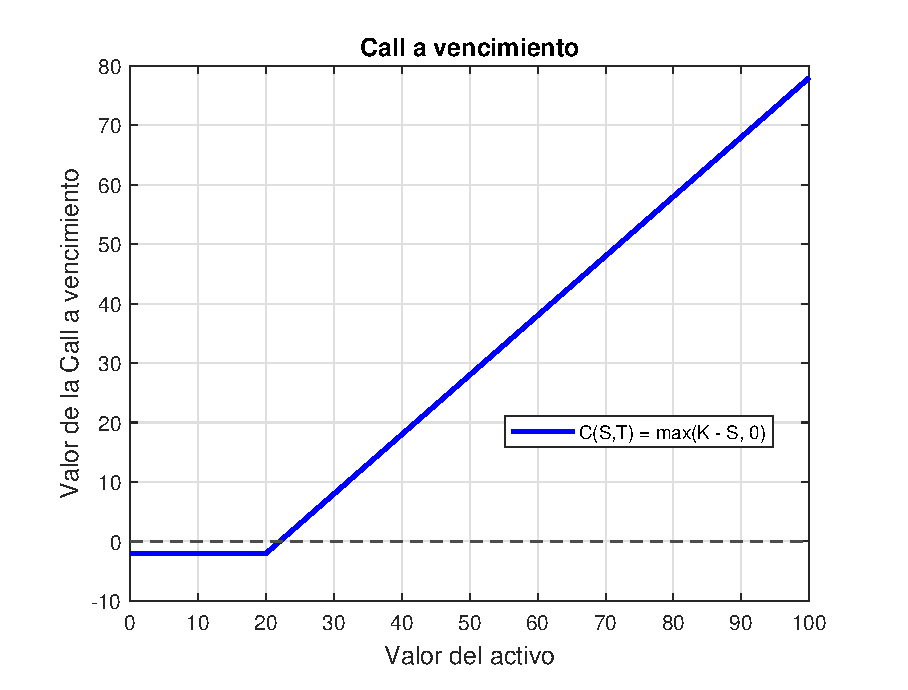
\includegraphics[width=\linewidth]{Imagenes/Parte1/2_Derivados/ProfitDiagCall.eps}
            \caption{Call option}
        \end{subfigure}
            \begin{subfigure}[b]{0.45\linewidth}
            \includegraphics[width=\linewidth]{Imagenes/Parte1/2_Derivados/ProfitDiagPut.eps}
            \caption{Put option}
        \end{subfigure}
        \caption{Profit diagram de opción a vencimiento}
    \end{figure}
    \item \textbf{Over the counter/OTC}: opciones que se realizan fuera de la bolsa y que no tienen que seguir las convenciones estándar. Los términos se especifican en una \textbf{term sheet}.
    \item \textbf{Gearing/leverage}: relación entre la posible ganancia y la inversión. Las opciones tienen una gran gearing, pero el punto negativo es que si no hay ganancias, la pérdida es del 100\% (se pierde la prima). Aquí el writer es el que tiene mucho riesgo.
    \item \textbf{Hedging}: tomar posiciones contrarias, por ejemplo ser el writer de una opción y comprar/vender acciones del subyacente para reducir riesgos. También se usa para describir la reducción de la aleatoriedad en general.
\end{itemize}



\subsection{Tipos de opciones}
\begin{itemize}
    \item \textbf{European options}: solo se puede ejercer en vencimiento.
    \item \textbf{American options}: se puede ejercer en cualquier momento hasta el vencimiento.
    \item \textbf{Bermudan options}: se puede ejercer en ciertas fechas específicas.
\end{itemize}


\subsection{Call-Put Parity}
La relación en cualquier tiempo $t$ entre una Call y una Put con los mismos parámetros es:
\[
    \boxed{C-P=S-Ke^{-r(T-t)}}
\]



\subsection{Opciones binarias/ digitales}
A fecha de ejercicio son discontinuas. Pagan una cierta cantidad fija (como un \$1) si el subyacente está por encima/debajo de cierto precio de ejercicio $E$ (o $K$). Las vainilla tienen un potencial de ganancia ilimitado, mientras que las binarias están acotadas, porque las compras cuando crees que el crecimiento/bajada es limitado.
\begin{figure}[H]
    \centering
    \begin{subfigure}[b]{0.45\linewidth}
        \includegraphics[width=\linewidth]{Imagenes/Parte1/2_Derivados/BinaryCall.eps}
        \caption{Call option}
    \end{subfigure}
        \begin{subfigure}[b]{0.45\linewidth}
        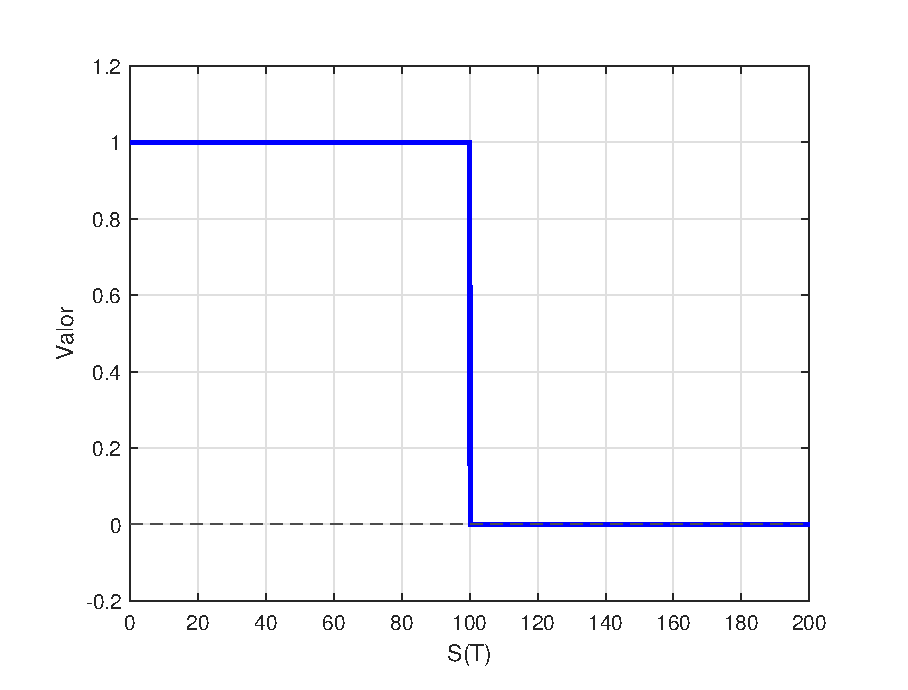
\includegraphics[width=\linewidth]{Imagenes/Parte1/2_Derivados/BinaryPut.eps}
        \caption{Put option}
    \end{subfigure}
    \caption{Binary option payoff}
\end{figure}
Su relación de paridad se obtiene considerando que tienes una opción binary de cada tipo, porque a precio de ejercicio se obtiene el \$1 que se paga (o la cantidad que se haya firmado) actualizado:
\[\text{Binary call} + \text{Binary put} = e^{-r(T-t)}\]




\subsection{Portfolio of options/Option strategy}
Conjunto de opciones combinadas de manera estratégica para un objetivo concreto (maximizar ganancias, minimizar riesgos,\dots). Para saber su payoff se suman los payoff de las opciones que compras y se restan los payoff de las opciones que vendes. De forma genérica, las estrategias se pueden clasificar en \textbf{spread} que son estrategias que involucran opciones del mismo tipo (calls o puts), y \textbf{combinations} que combinan opciones de distinto tipo (calls o puts); también existen las \textbf{calendar spread}, que combinan opciones con distintas fechas de vencimiento. Algunos ejemplos son:
\begin{itemize}
    \item \textbf{Bull Spread (Spread Alcista)}: consiste en comprar una opción \textbf{call} con un strike más bajo $E_1$ y veneder otra opción call con strike más alto $E_2$  ($E_1<E_2$). Hay beneficio si subyacente \textbf{sube}, pero está limitado a diferencia $E_2-E_1$. Su payoff es:
    \[\boxed{\max(S-E_1, 0) - \max(S-E_2, 0)}\]
    \begin{figure}[H]
        \centering
        \includegraphics[width=0.5\linewidth]{Imagenes/Parte1/2_Derivados/BullPayoff.eps}
        \caption{Payoff de Bull Spread a vencimiento (normalizado)}
    \end{figure}
    Para normalizarlo se divide por $E_2-E_1$
    \item \textbf{Bear Spread (Spread Bajista)}: consiste consiste en comprar opción \textbf{put} con strike más alto $E_2$ y vender otra con strike más bajo $E_1$ ($E_1<E_2$). Hay beneficio si el subyacente \textbf{baja}, pero está limitado a diferencia $E_2-E_1$. Su payoff es:
     \[\boxed{\max(E_2-S, 0) - \max(E_1-S, 0)}\]
    \begin{figure}[H]
        \centering
        \includegraphics[width=0.5\linewidth]{Imagenes/Parte1/2_Derivados/BearPayoff.eps}
        \caption{Payoff de Bear Spread a vencimiento (normalizado)}
    \end{figure}
    Para normalizarlo se divide por $E_2-E_1$
    \item \textbf{Straddles}: comprar una call y una put con mismo strike y mismo expirity. Beneficio depende de la magnitud del movimiento del subyacente, pero costo alto por primas de dos opciones. Se suele hacer cuando hay un anuncio importante. Su payoff es:
    \[\boxed{\max(S-E, 0) + \max(E-S, 0)}\]
    \begin{figure}[H]
        \centering
        \includegraphics[width=0.5\linewidth]{Imagenes/Parte1/2_Derivados/StraddlePayoff.eps}
        \caption{Payoff de Straddle}
    \end{figure}
    \item \textbf{Strangle}: similar a straddles, pero con strikes distintos. Es más barato pero precisa de mayores cambios en el subyacente para que haya beneficios. Su payoff es:
    \[\boxed{\max(S-E_C, 0) + \max(E_P-S, 0)}\]
    Según los strikes pueden ser:
    \begin{itemize}
        \item \textbf{Out-of-the-Money Strangle (OTM)}: se compra call con strike por encima de precio actual y put con strike por debajo de actual. Es más barato (primas bajas) pero se necesita un movimiento grande del subyacente.
        \begin{figure}[H]
            \centering
            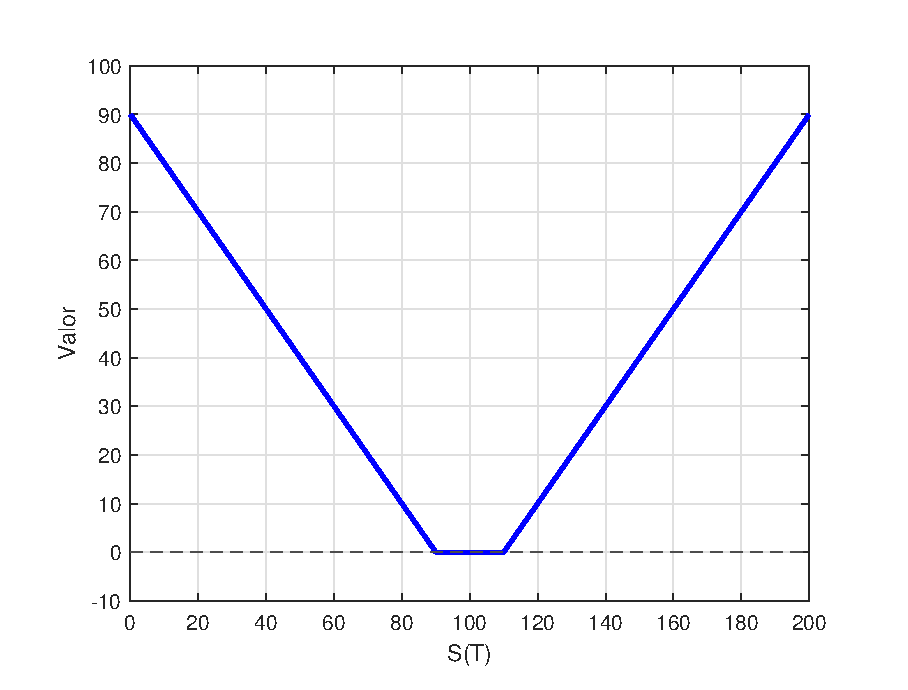
\includegraphics[width=0.5\linewidth]{Imagenes/Parte1/2_Derivados/StrangleOTMPayoff.eps}
            \caption{Payoff de Strangle OTM}
        \end{figure}
        \item \textbf{In-the-Money Strangle (ITM)}: se compra call con strike por debajo de precio actual y put con strike por encima de actual. Algo más caro (por primas) que OTM, pero un poco más seguro.
        \begin{figure}[H]
            \centering
            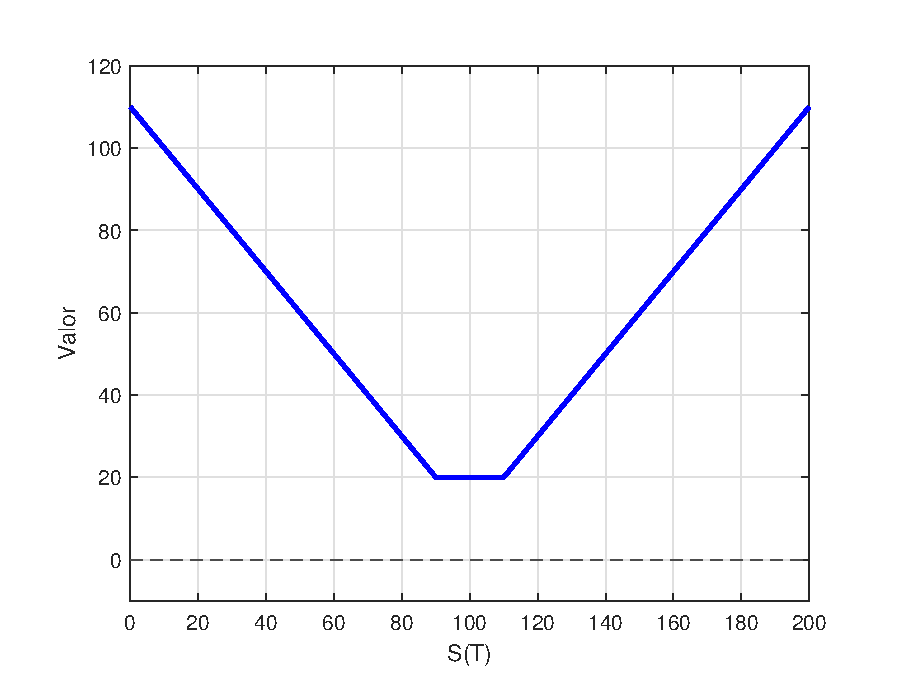
\includegraphics[width=0.5\linewidth]{Imagenes/Parte1/2_Derivados/StrangleITMPayoff.eps}
            \caption{Payoff de Strangle ITM}
        \end{figure}
    \end{itemize}
    \item \textbf{Risk Reversal}: comprar una call con strike mayor que el precio actual y vender una put con un strike inferior al precio actual. Se apuesta a que el subyacente va a subir (y que como mucho no va a bajar demasiado). Si el activo baja se pierde dinero, pero las primas son más baratas. Su payoff sería:
    \[\boxed{\max(S-E_C, 0) - \max(E_P-S, 0)}\]
    \begin{figure}[H]
        \centering
        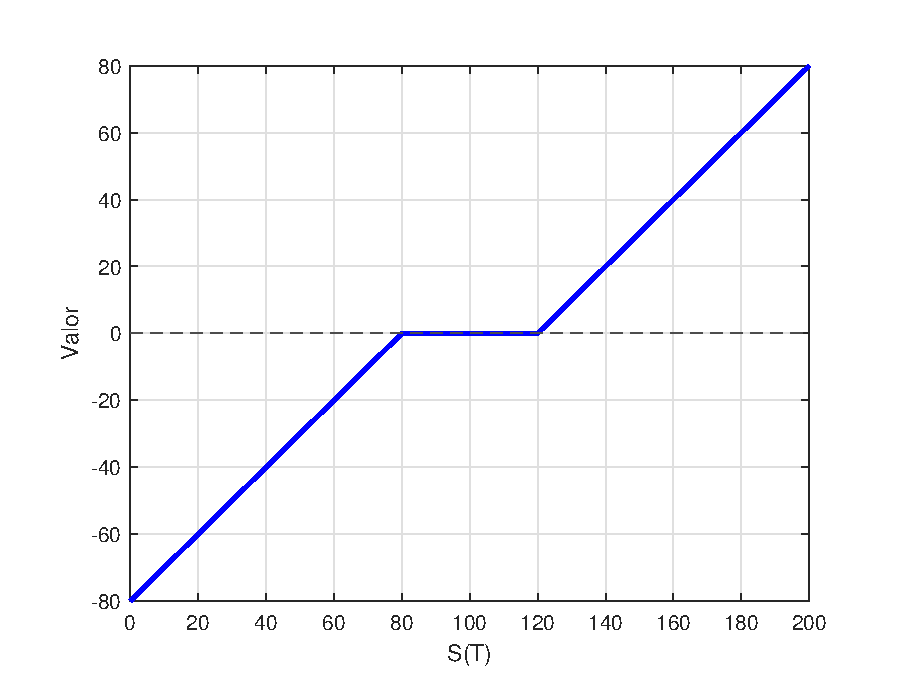
\includegraphics[width=0.5\linewidth]{Imagenes/Parte1/2_Derivados/RiskReversalPayoff.eps}
        \caption{Payoff de Risk Reversal a vencimiento}
    \end{figure}
    \item \textbf{Butterflies}: se compra una call ITM ($E_{C_{ITM}}$), se venden dos calls ATM (at-the-money) ($E_{C_{ATM}}$) y se compra una call OTM ($E_{C_{OTM}}$). Es decir, $E_{C_{ITM}}<E_{C_{ATM}}<E_{C_{OTM}}$. Además, generalmente se cumple que $E_{C_{OTM}} - E_{C_{ATM}} = E_{C_{ATM}} - E_{C_{ITM}}$. Se usa cuando se espera que el subyacente esté cerca de cierto precio central y haya poca volatilidad. Su payoff es:
    \[\boxed{\max(S-E_{C_{ITM}}, 0) - 2\max(S-E_{C_{ATM}}, 0) + \max(S-E_{C_{OTM}}, 0)}\]
    \begin{figure}[H]
        \centering
        \includegraphics[width=0.5\linewidth]{Imagenes/Parte1/2_Derivados/ButterflyPayoff.eps}
        \caption{Payoff de Butterfly a vencimiento}
    \end{figure}
    \item \textbf{Condors}: parecido a butterflies, se compra call con strike $E_1$, se vende call con strike $E_2$, se vende call con strike $E_3$, y se compra call con strike $E_4$ tal que $E_1<E_2<E_3<E_4$. Además, generalmente se cumple que $E_2-E_1=E_4-E_3$. Se obtienen ganancias máximas si el subyacente se mantiene entre $E_2$ y $E_3$. Su payoff es:
    \[\boxed{\max(S-E_1, 0) - \max(S-E_2, 0) - \max(S-E_3, 0) + \max(S-E_4, 0)}\]
    \begin{figure}[H]
        \centering
        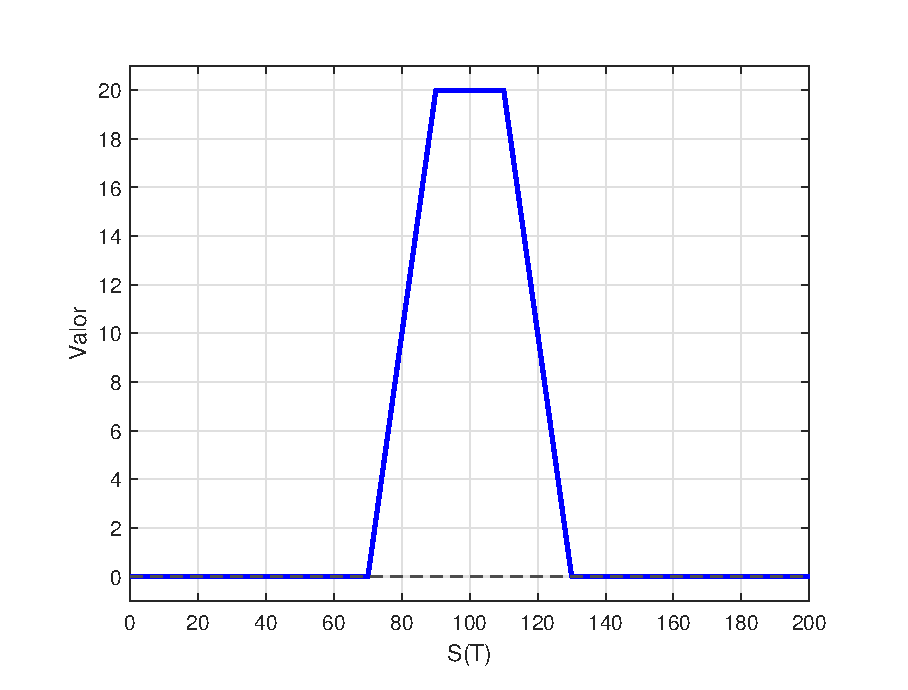
\includegraphics[width=0.5\linewidth]{Imagenes/Parte1/2_Derivados/CondorsPayoff.eps}
        \caption{Payoff de Condors a vencimiento}
    \end{figure}
\end{itemize}



\subsection{Opciones a largo plazo}
\begin{itemize}
    \item \textbf{LEAPS/ long-term equity anticipation securities}: opciones con hasta 3 años de fecha de vencimiento. Usualmente vencen en enero. Se suelen emitir a 3 precios de ejercicio: ATM (precio actual), 20\% ITM (más favorable para el comprador) o 20\% OTM (más especulativo).
    \item \textbf{FLEX/ FLexible EXchange-traded options}: permiten más personalización de la opcion de la fecha de vencimiento (hasta 5 años), el strike o el tipo de ejercicio (europeo o americano).
\end{itemize}


\subsection{Otros derivados}
\begin{itemize}
    \item \textbf{Warrants}: parecido a opciones call, pero emitido por la propia empresa del subyacente que da derecho a comprar acciones \textit{nuevas} (frente a acciones ya existentes en las opciones) emitidas por la empresa. Tiene plazos largos, de hasta 5 años.
    \item \textbf{Convertible bonds/ CBs}: bono normal que paga cupones y un capital a vencimiento, pero que tiene la opción de convertirse en acciones antes de vencimiento (perderías los cupones siguientes). Se comporta como una opción americana.
\end{itemize}











\newpage

\section{Algunas propiedades}

\subsection{Desigualdad de Jensen}
Sea la función convexa $f(S)$ (que se curva hacia arriba, con forma de cuenco) de la variable aleatoria $S$, entonces
\[\mathbb{E}[f(S)] \geq f(\mathbb{E}[S])\]
De hecho, la diferencia es de
\[\frac{1}{2}f''(\mathbb{E}[S])\mathbb{E}[\epsilon]\]
donde $\epsilon$ es la desviación de $S$ de la media, i.e $S=\mathbb{E}[S]+\epsilon$.


\subsection{Propiedad de Markov}
\textit{El futuro depende solo del presente, no del pasado.} Se usa en los caminos aleatorios para decir que el valor $S_t+1$ solo depende de $S_t$, es decir,
\[\mathbb{P}(X_{t+s} \in A \mid X_t = x, X_{t_1} = x_1, \ldots, X_{t_n} = x_n) 
= \mathbb{P}(X_{t+s} \in A \mid X_t = x)\]



\subsection{Propiedad de martingala}
\textit{Lo que esperas tener en el futuro, sabiendo todo hasta ahora, es exactamente lo que tienes ahora}. Es decir, el valor esperado de algo en un juego justo es exactamente lo que tienes ahora:
\[\mathbb{E}[S_i|S_j, j<i]=S_j\]



\subsection{Lema de Itô}
Sea
\[dS = a(S,t)dt + b(S,t)d\mathnormal{X}\]
entonces
\begin{equation}
    \boxed{dV = \left( \frac{dV}{dt} + \frac{1}{2}b^2\frac{d^2V}{dS^2} \right)\,dt + \frac{dV}{dS}\,dS = \left( \frac{dV}{dt} +  a\frac{dV}{dS} + \frac{1}{2}b^2\frac{d^2V}{dS^2} \right)\,dt + b\frac{dV}{dS}\,d\mathnormal{X}}
\end{equation}\label{Ito}
En el apéndice~\ref{CalcIto} se encuentra la fórmula para dimensiones mayores. Para el caso en el que se tenga varios procesos correlacionados, la fórmula de Ito se puede escribir como:
\begin{equation}\label{eq:ItoCorrelated}
    \boxed{dV = \left( \frac{\partial V}{\partial t} + \frac{1}{2} \sum_{i=1}^{d} \sum_{j=1}^{d} b_i b_j \rho_{ij} \frac{\partial^2 V}{\partial S_i \partial S_j} \right)\,dt + \sum_{i=1}^{d} \frac{\partial V}{\partial S_i}\,dS_i}
\end{equation}

\subsection{Algunos ejemplos de caminos aleatorios}

\begin{itemize}
    \item \textbf{Brownian Motion with Drift}: $\boxed{dS = \mu dt + \sigma d\mathnormal{X}}$
    \begin{figure}[H]
        \centering
        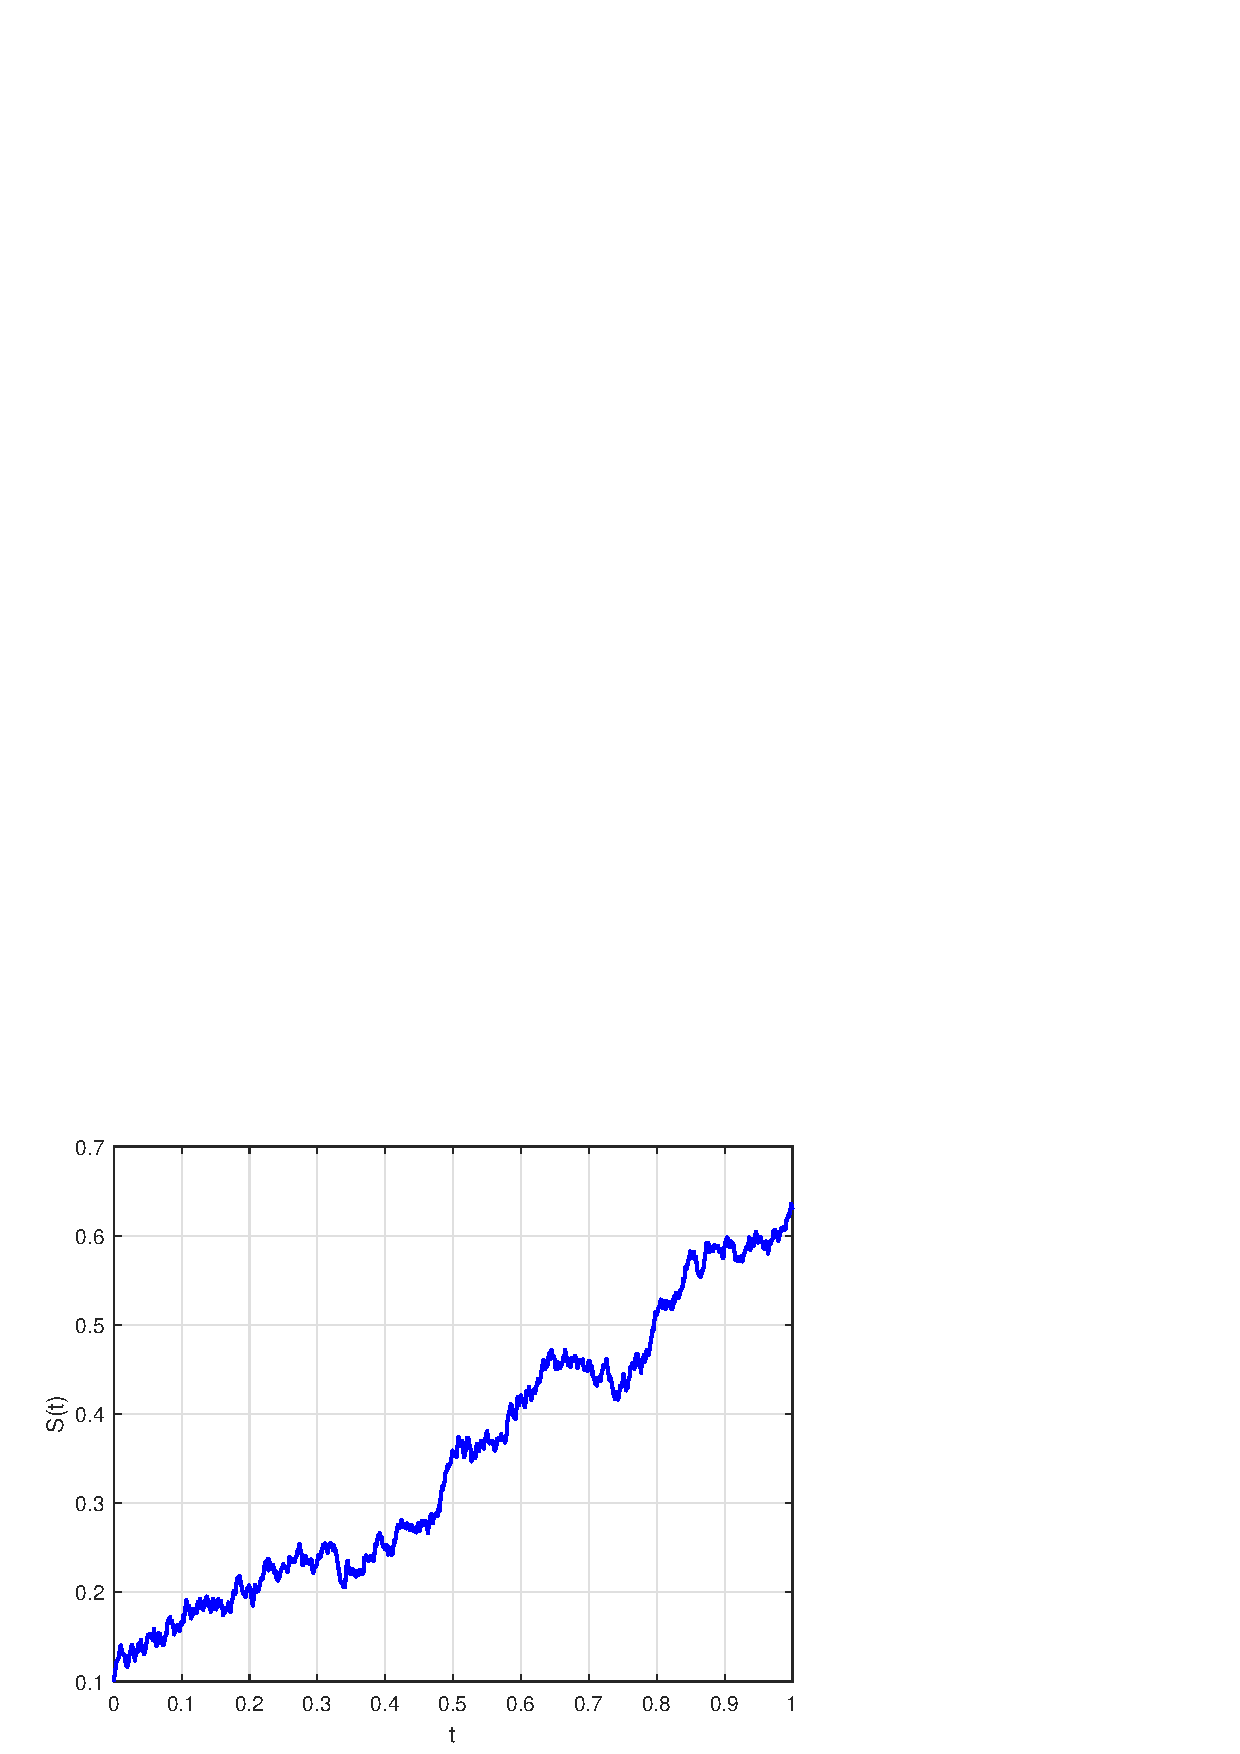
\includegraphics[width=0.65\linewidth]{Imagenes/Parte1/3_Aleatoriedad/BrownianMotionDrift.pdf}
        \caption{Brownian Motion with Drift}
    \end{figure}
    \item \textbf{The Lognormal Random Walk}: $\boxed{dS = S\mu dt + S\sigma d\mathnormal{X}}$
    \begin{figure}[H]
        \centering
        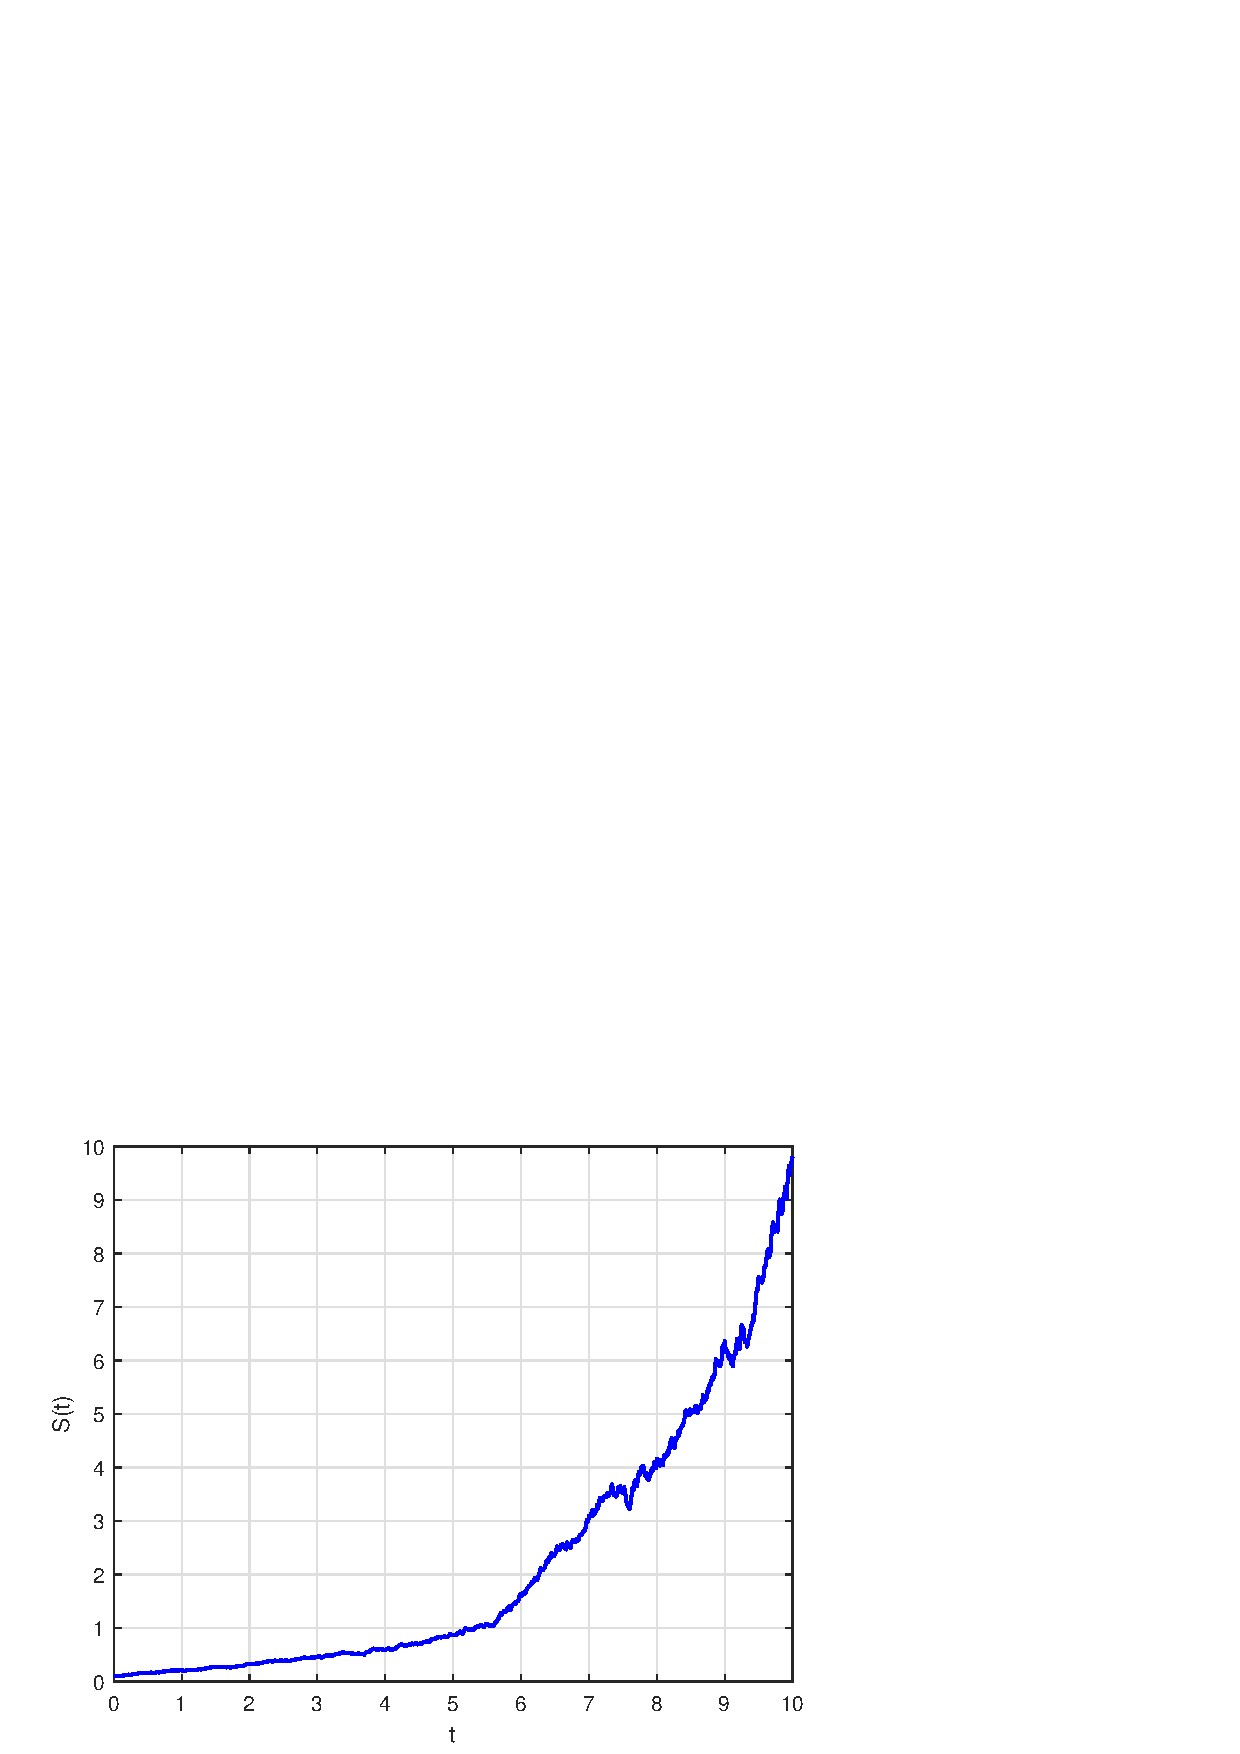
\includegraphics[width=0.65\linewidth]{Imagenes/Parte1/3_Aleatoriedad/LognormalRandomWalk.pdf}
        \caption{The Lognormal Random Walk}
    \end{figure}
    \item \textbf{A Mean-reverting Random Walk}: reversion a la media, cuando se esta fuera del crecimiento normal el camino tiende a corregirse.\\
    Su EDE es 
    \[
        \boxed{dS = \kappa(\theta-S) dt + \sigma d\mathnormal{X}}
    \]
    donde $\kappa$ es la velocidad de reversión a la media, $\theta$ es la tasa de interés a largo plazo y $\sigma$ es la volatilidad. Un ejemplo común es el modelo Vasicek para el ratio de interés, $dr = \kappa(\theta+r) dt + \sigma d\mathnormal{X}$
    \begin{figure}[H]
        \centering
        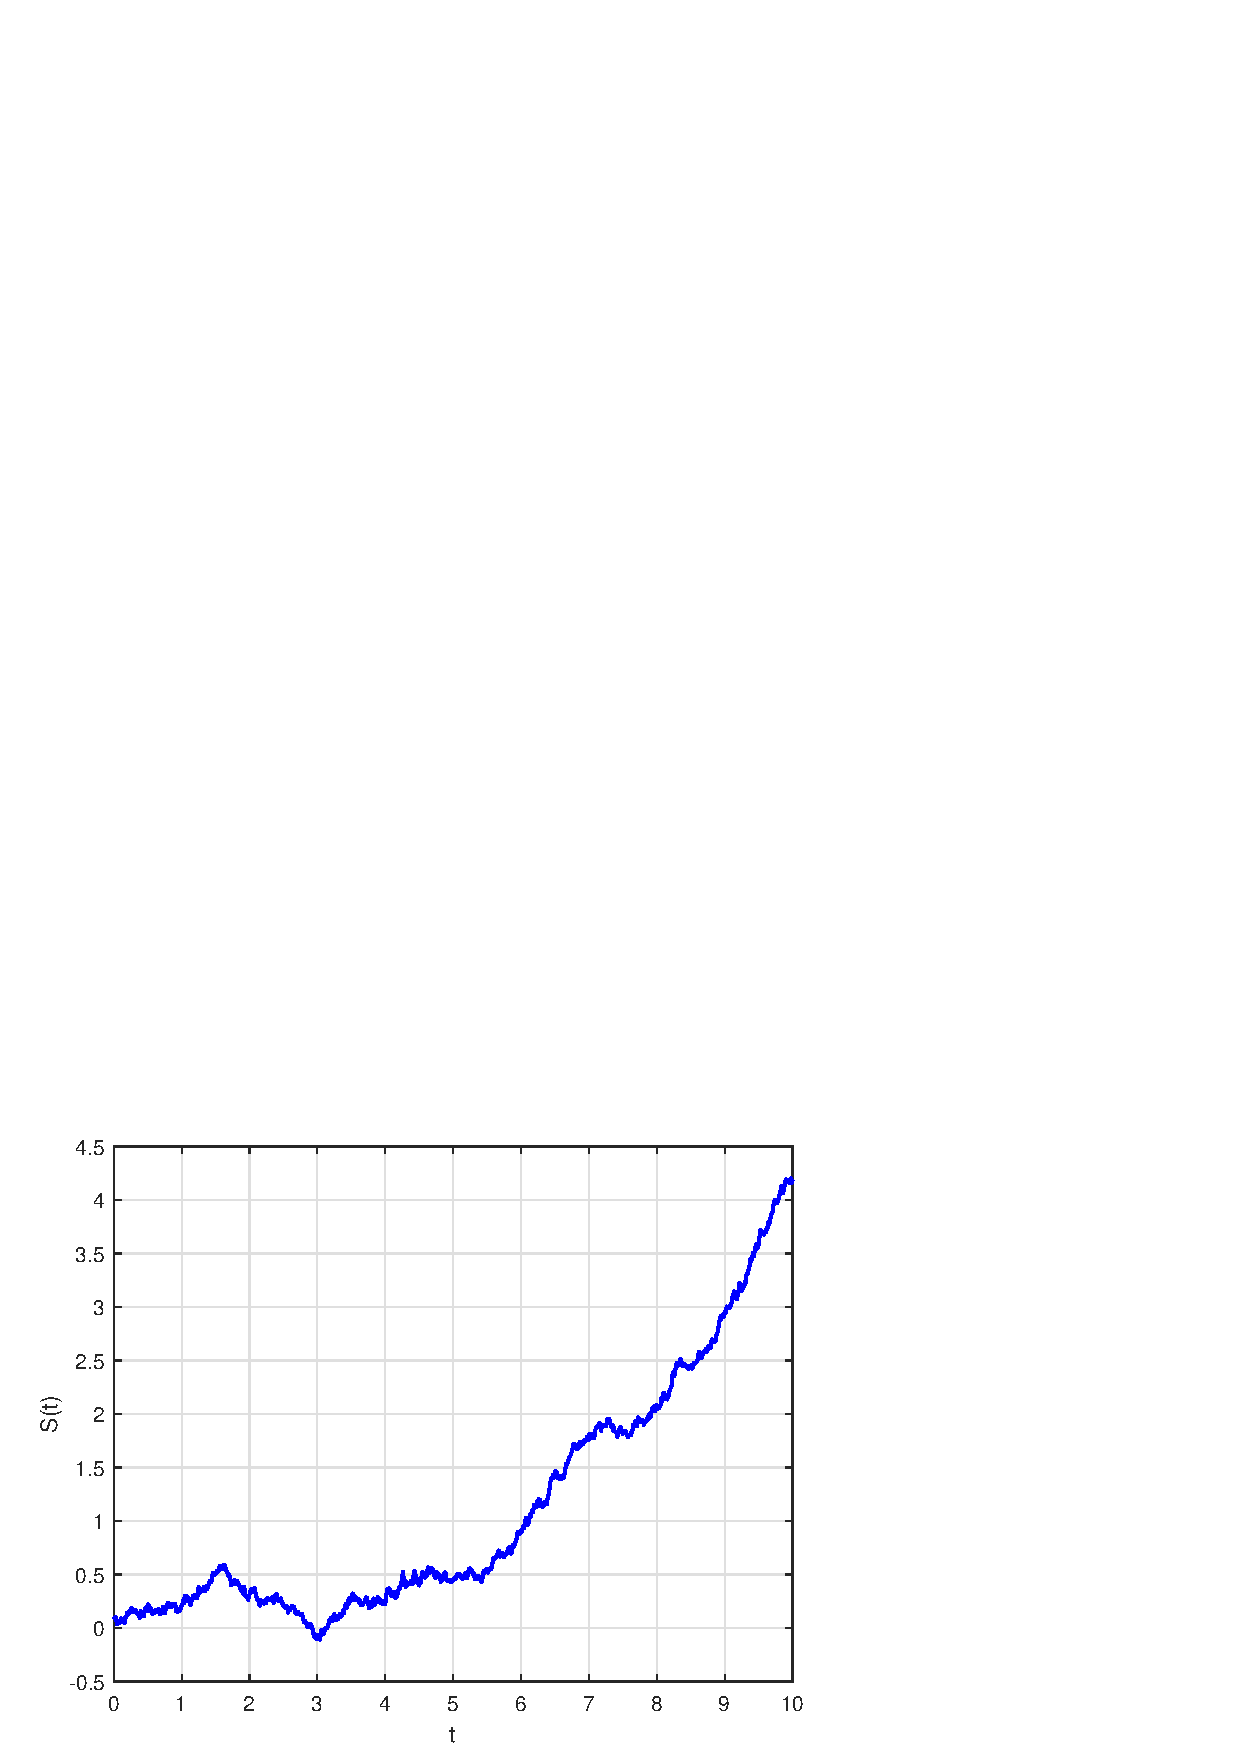
\includegraphics[width=0.65\linewidth]{Imagenes/Parte1/3_Aleatoriedad/MeanRevertingWalk.pdf}
        \caption{Mean-reverting Random Walk}
    \end{figure}
\end{itemize}



\section{Función de densidad de transición}
Es la \textit{`probabilidad de que una variable aleatoria $y$ esté entre $a$ y $b$ en el instante futuro $t'$, sabiendo que ha empezado con un valor $y$ en el instante $t$`}. En concreto la función de densidad de transición $p(y, t; y', t')$ es:
\[
    \boxed{\text{Prob}(a<y'<b\text{ en }t' | y\text{ en }t) = \int_a^b p(y, t; y', t') dy'}
\]

\subsection{Ecuación de Fokker-Planck o de Kolmogorov hacia delante}
Se centra en cómo evoluciona la transición con respecto al tiempo futuro $t'$. Se enfoca en el destino del proceso y cómo cambia la probabilidad de estar en distintos valores futuros $y'$ a medida que avanza el tiempo $t'$. Esta ecuación se usa cuando hay un espacio especial ahora y se quiere saber que va a pasar en el futuro. Sabiendo que la variable aleatoria cumple la EDE
\[
    dy = A(y, t) dt + B(y, t) d\mathnormal{X}
\]
entonces la función de densidad de transición es la solución de la ecuación diferencial parcial
\[
    \boxed{\frac{\partial p}{\partial t'} = \frac{1}{2} \frac{\partial^2}{\partial y'^2} \left( B(y', t')^2 p \right) - \frac{\partial}{\partial y'} \left( A(y', t') p \right)}
\]
por ejemplo para la EDE
\[
    dS = \mu S dt + \sigma S d\mathnormal{X}
\]
se tiene que reolver la EDP
\[
    \frac{\partial p}{\partial t'} = \frac{1}{2} \frac{\partial^2}{\partial S'^2} \left( \sigma^2 S'^2 p \right) - \frac{\partial}{\partial S'} \left( \mu S' p \right)
\]
que da como solución
\[
    p(S, t; S', t') = \frac{1}{\sigma S' \sqrt{2\pi (t'-t)}} \exp\left( -\frac{ \left( \log(S/S') + (\mu - \frac{1}{2}\sigma^2)(t'-t) \right)^2 }{ 2\sigma^2 (t'-t) } \right)
\]
\begin{figure}[H]
    \centering
    \begin{subfigure}[b]{0.45\linewidth}
        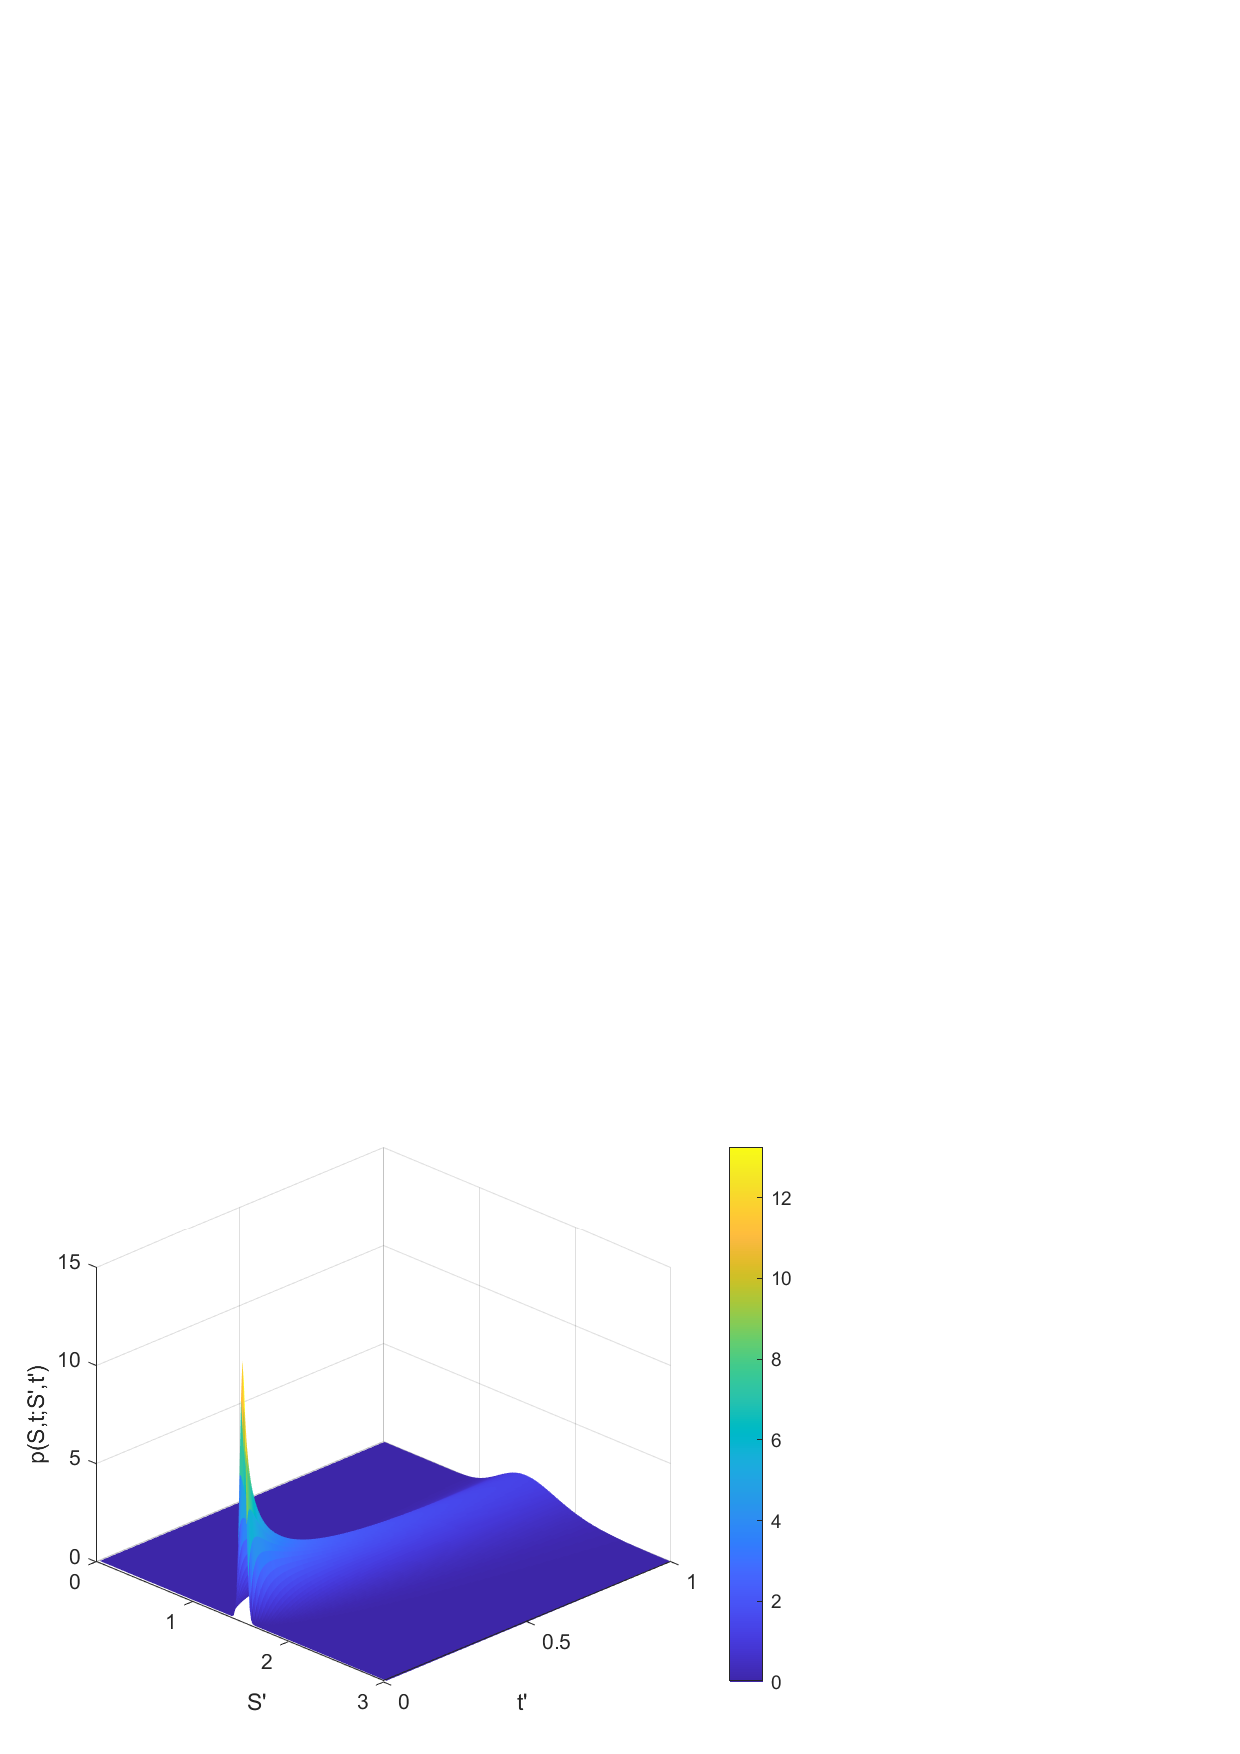
\includegraphics[width=\linewidth]{Imagenes/Parte1/3_Aleatoriedad/PDF_3D.pdf}
    \end{subfigure}
        \begin{subfigure}[b]{0.45\linewidth}
        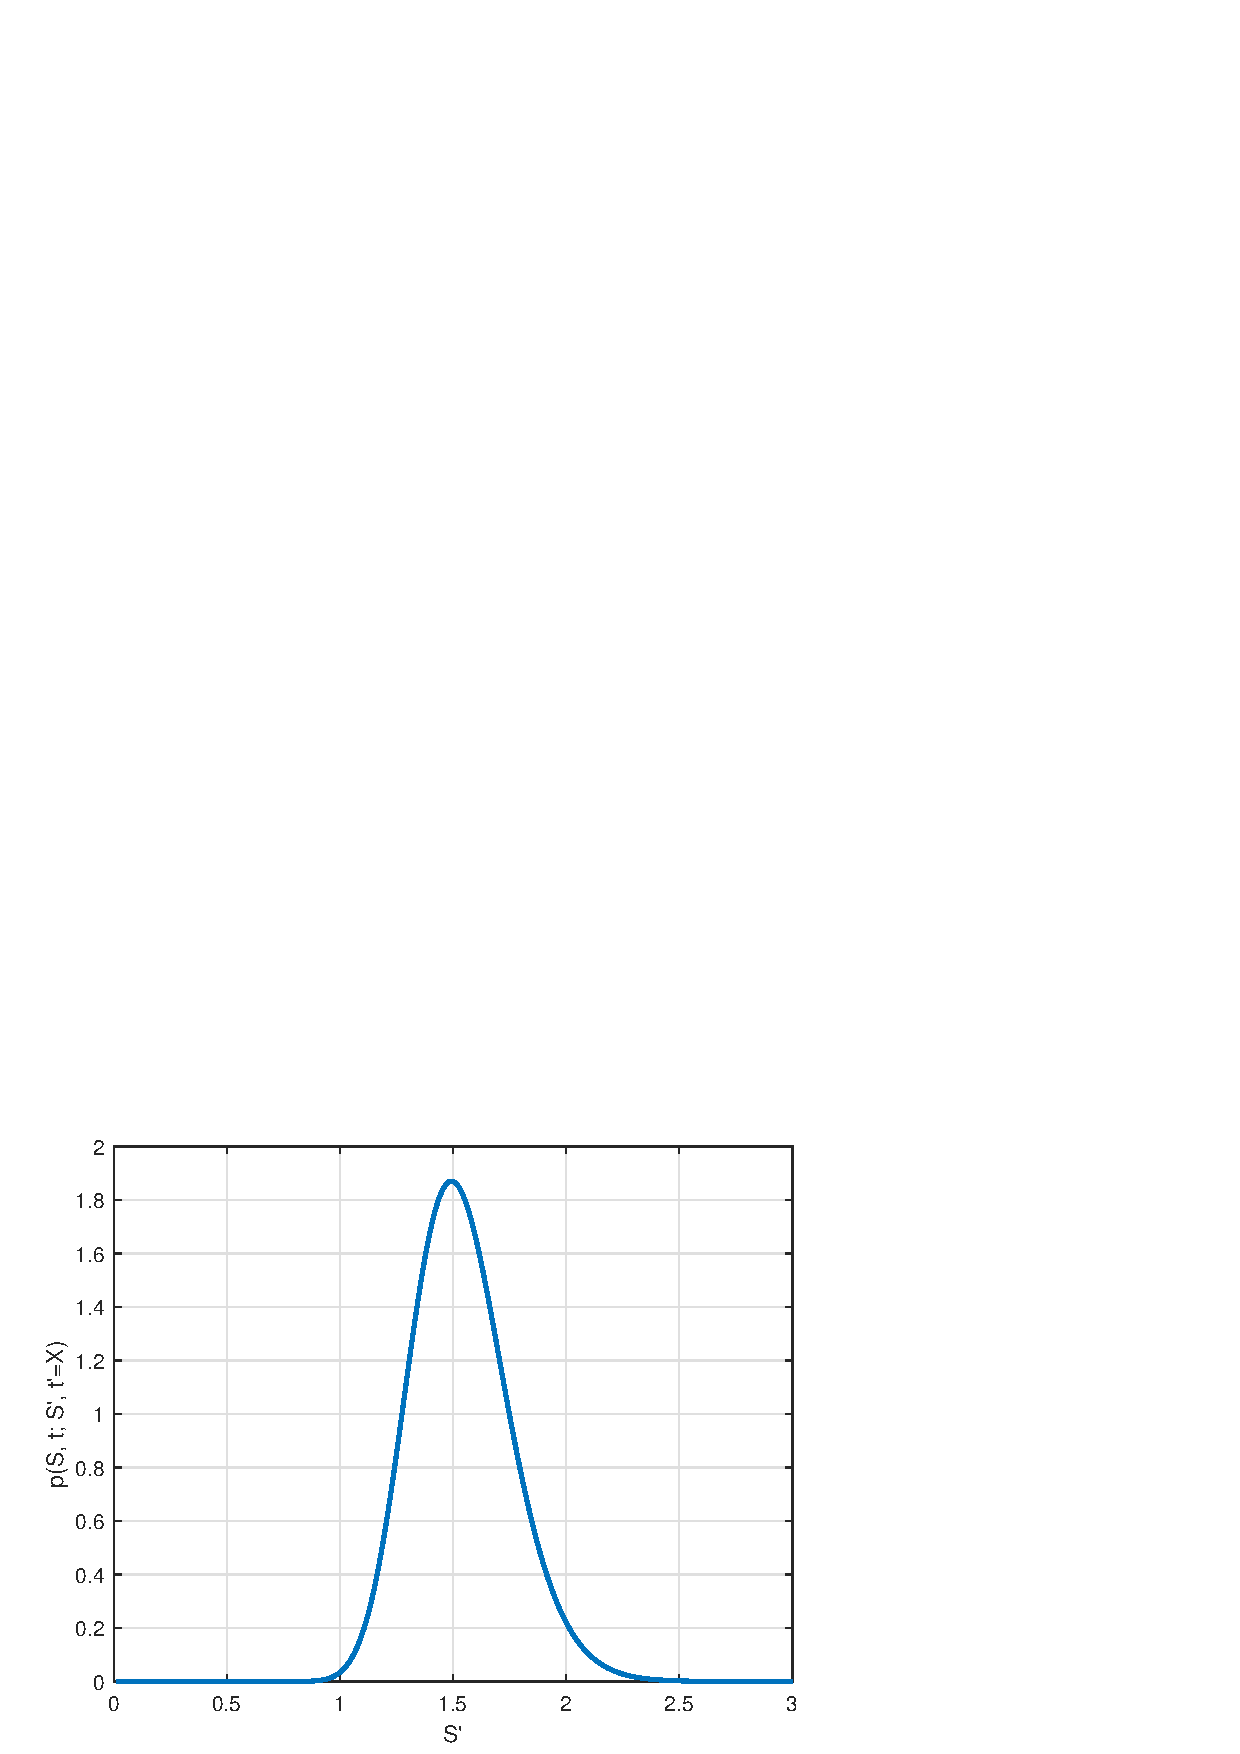
\includegraphics[width=\linewidth]{Imagenes/Parte1/3_Aleatoriedad/PDF_2D.pdf}
    \end{subfigure}
    \caption{Función de densidad de transición}
\end{figure}



\subsubsection{Ecuación de Kolmogorov hacia detrás}\label{sec:KolmogorovDetras}
Se centra en cómo evoluciona la densidad de transición con respecto al tiempo actual $t$. Se enfoca más en el origen  y cómo cambian las probabilidades de llegar al punto $y'$, $t'$ dependiendo de donde se está en el momento. La EDP es
\[
    \boxed{\frac{\partial p}{\partial t} + \frac{1}{2} B(y, t)^2 \frac{\partial^2 p}{\partial y^2} + A(y, t) \frac{\partial p}{\partial y} = 0}
\]


\subsubsection{Distribución en estado estacionario (steady-state distribution)}
Son aquellas cuya función de densidad de transición $p(y, t; y', t')$ tiende, cuando $t' \to \infty$, a una distribución que ya no depende del estado inicial $y$ ni del tiempo $t$. Para eso se debe cumplir que el proceso sea homogéneo en el tiempo, i.e. $A$ y $B$ sean independientes de $t$ en el límite asintótico. Cuando se cumple la función de densidad de transición converge a $p_\infty(y')$ que satisface:
\[
    \boxed{\frac{1}{2} \frac{d^2}{dy'^2} \left( B_\infty^2 p_\infty \right) - \frac{d}{dy'} \left( A_\infty p_\infty \right) = 0}
\]
donde $A_\infty$ y $B_\infty$ son los valores de los coeficientes en el límite $t \to \infty$.








\section{Tiempos de primer escape (First-exit times)}\label{sec:FirstExitTimes}
El \textit{first-exit time} es el tiempo en el cual un camino aleatorio alcanza un cierto límite por primera vez. El objetivo de esta sección es calcular la probabilidad de que un camino aleatorio alcance cierto límite antes de cierto tiempo.
\begin{figure}[H]
    \centering
    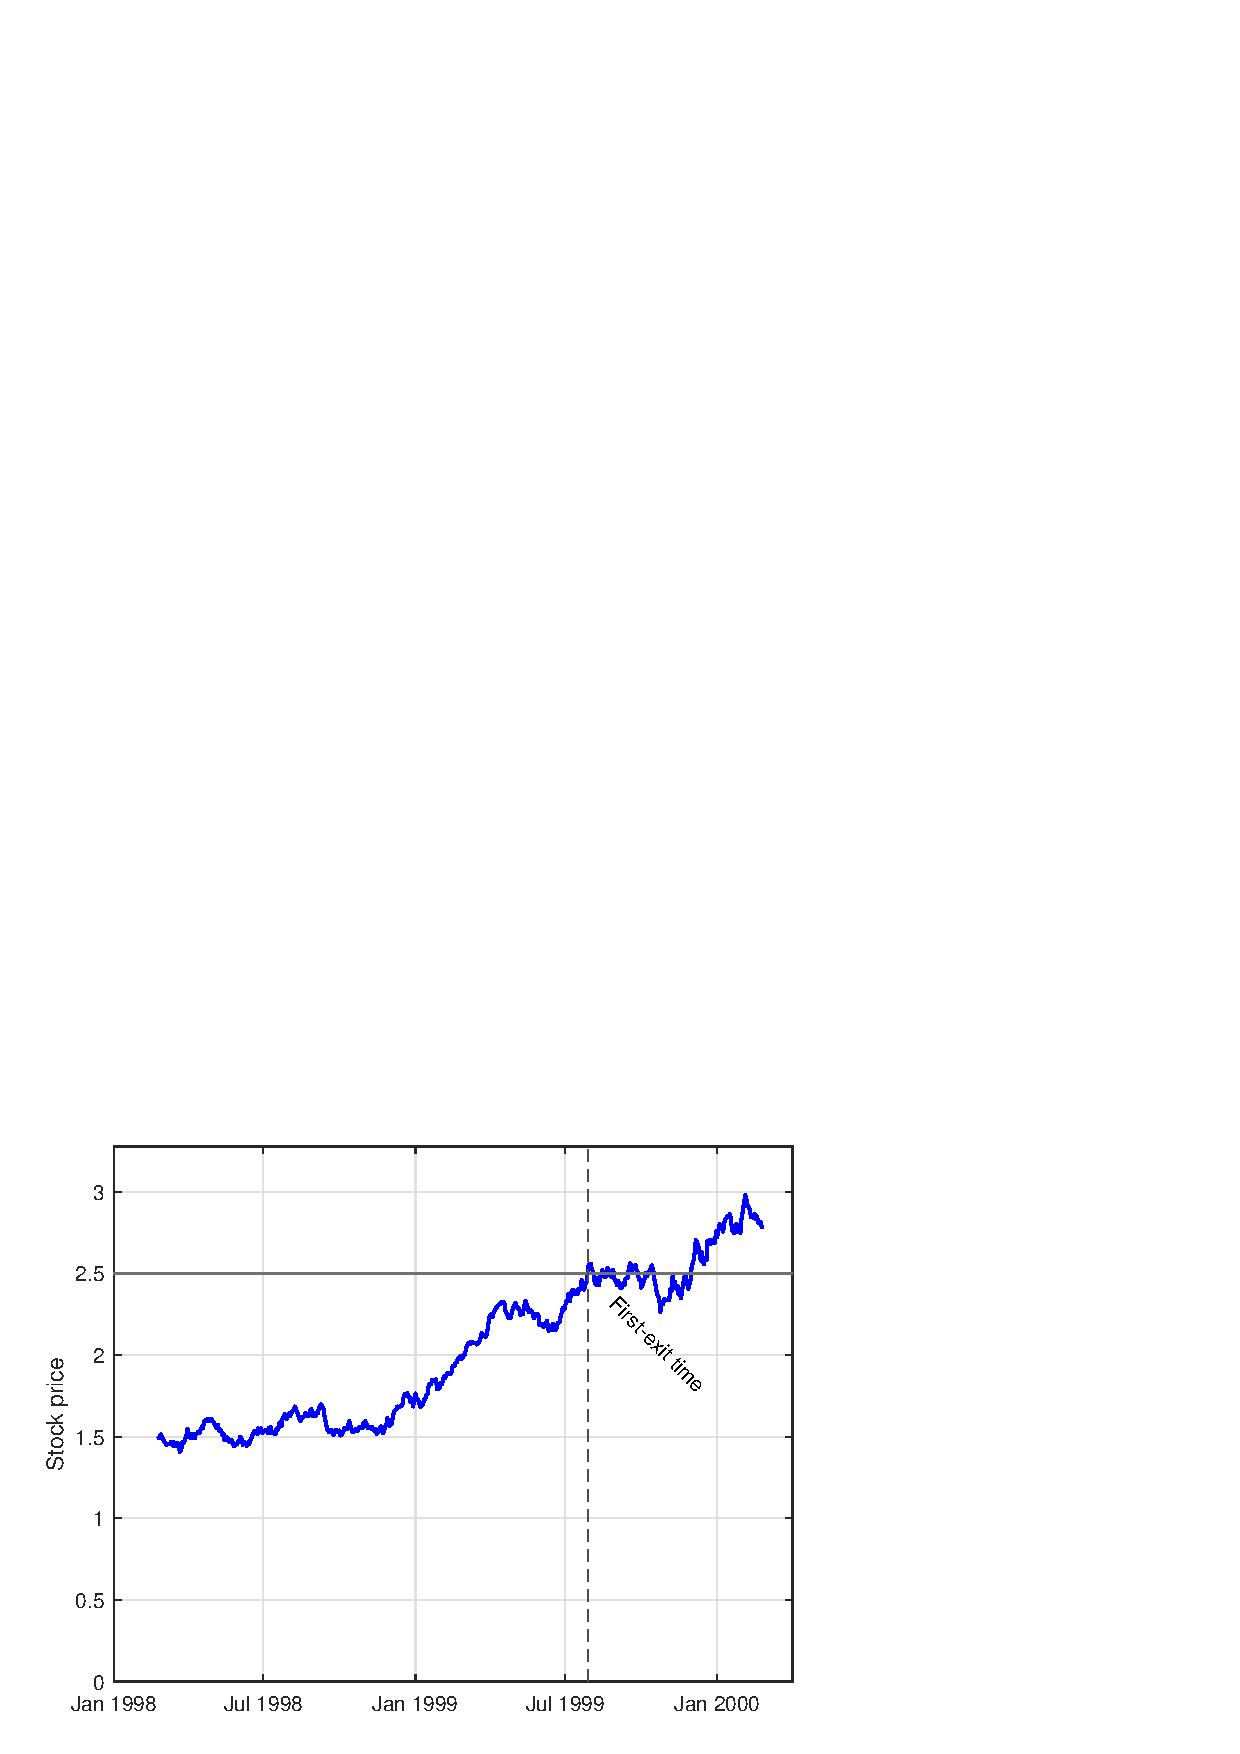
\includegraphics[width=0.65\linewidth]{Imagenes/Parte1/3_Aleatoriedad/First-exit_Time.pdf}
    \caption{First-exit Time}
\end{figure}




\subsection{Funciones de distribución acumulada para first-exit times}
Se definde la función $C(y, t; t')$ como la probabilidad de que la variable $y$ salga de la región $\Omega$ antes del tiempo $t'$, habiendo empezado en $y$ en el tiempo $t$. Esta función puede interpretarse como una función de distribución acumulada para first-exit time. 

El objetivo es calcular la probabilidad de que un camino aleatorio abandone una región $\Omega$ antes de un tiempo dado $t'$. Para ello, se tiene que satisfacer el problema de la EDP hacia atrás:
\begin{equation}\label{eq:CumulatFirstExitTime}
    \boxed{
    \left\{
    \begin{array}{rlrl}
        \displaystyle\frac{\partial C}{\partial t} + \frac{1}{2} B(y, t)^2 \frac{\partial^2 C}{\partial y^2} + A(y, t) \frac{\partial C}{\partial y} = 0 &\quad& (y,t) \in \Omega\times(0, t') \\[2ex]
        C(y, t; t') = 1 && (y,t) \in \partial\Omega\times(0, t') \\[2ex]
        C(y, t'; t') = 0 && y \in \Omega \\
    \end{array}
    \right\}
    }
\end{equation}




\subsection{Tiempos de primer escape esperados (Expected first-exit times)}\label{sec:ExpectedFirstExitTimes}
Una vez calculado~\eqref{eq:CumulatFirstExitTime} es posile calcular el tiempo esperado de primer escape:
\[
    u(y, t) = \int_t^\infty (t' - t) \frac{\partial C}{\partial t'} dt' \overset{\text{partes}}{=} \int_t^\infty 1 - C(y, t; t') dt'
\]
por lo tanto,
\begin{align*}
    \frac{\partial u}{\partial t}  &= \frac{\partial}{\partial t} \left(\int_t^\infty 1 - C(y, t; t') dt' \right) \overset{\text{Leibniz}}{=} -\left(1-C(y, t, t)\right) + \int_t^\infty \frac{\partial}{\partial t}\left(1 - C(y, t; t')\right) dt' \\
    &\overset{\text{\eqref{eq:CumulatFirstExitTime}}}{=} -1 - \int_t^\infty \frac{\partial}{\partial t} C(y, t; t') dt' \\
    \frac{\partial u}{\partial y}  &= \int_t^\infty \frac{\partial}{\partial y}\left(1 - C(y, t; t')\right) dt' = - \int_t^\infty \frac{\partial}{\partial y} C(y, t; t') dt' \\
    \frac{\partial^2 u}{\partial y^2}  &= - \int_t^\infty \frac{\partial^2}{\partial y^2} C(y, t; t') dt' \\
\end{align*}
que volviendo a la EDP~\eqref{eq:CumulatFirstExitTime}:
\begin{align*}
    &\int_t^\infty\frac{\partial C}{\partial t} + \frac{1}{2} B(y, t)^2 \frac{\partial^2 C}{\partial y^2} + A(y, t) \frac{\partial C}{\partial y} dt' = 0 \Rightarrow \\
    &\Rightarrow \int_t^\infty\frac{\partial C}{\partial t} dt' + \frac{1}{2} B(y, t)^2 \int_t^\infty \frac{\partial^2 C}{\partial y^2} dt' + A(y, t) \int_t^\infty \frac{\partial C}{\partial y} dt' = 0 \Rightarrow \\
    &\Rightarrow -1 - \frac{\partial u}{\partial t} - \frac{1}{2} B(y, t)^2 \frac{\partial^2 u}{\partial y^2} - A(y, t) \frac{\partial u}{\partial y} = 0
\end{align*}
por lo que el tiempo esperado de primer escape $u(y, t)$ satisface la EDP
\[
    \boxed{
        \left\{
        \begin{aligned}
            \frac{\partial u}{\partial t} + \frac{1}{2} B(y, t)^2 \frac{\partial^2 u}{\partial y^2} + A(y, t) \frac{\partial u}{\partial y} = -1\\
            u(y, t) = 0 && y \in \partial\Omega \\
        \end{aligned}
        \right\}
    }
\]
Por ejemplo, si se tiene una EDE independiente del tiempo $A=\mu S, B=\sigma S$, se puede buscar una solución en estado estacionario, es decir, $u(y, t) = u(y)$, que satisface la EDP
\[
    \frac{1}{2}\sigma^2 S^2 \frac{d^2 u}{dS^2} + \mu S \frac{du}{dS} = -1
\]
con condiciones de contorno $u(S_0) = u(S_1) = 0$. La solución en este caso sería.
\[
    u(S) = \frac{1}{\frac{1}{2}\sigma^2 - \mu} \left( \log(S/S_0) - \frac{1 - (S/S_0)^{1-2\mu/\sigma^2}}{1 - (S_1/S_0)^{1-2\mu/\sigma^2}} \log(S_1/S_0) \right)
\]








\section{Estrategias en apuestas}

\subsection{Blackjack}
La distribución del beneficio en el blackjack (explicado en el apéndice~\ref{sec:blackjack}) es la siguiente. Se denota $\phi$ a la variable aleatoria que represestan el resultado de la apuesta, $\mu$ es la media de y $\sigma$ es la desviación típica de $\phi$. En blackjack, los valores discretos de $\phi$ son:
\begin{align*}
    &\phi = -1, && \text{el jugador pierde la apuesta} \\
    &\phi = 0, && \text{el jugador empata} \\
    &\phi = 1, && \text{el jugador gana la apuesta} \\
    &\phi = 3/2, && \text{el jugador consigue un blackjack o natural} \\
\end{align*}
\begin{figure}[H]
    \centering
    \includegraphics[width=0.65\linewidth]{Imagenes/Parte1/3_Aleatoriedad/blackjack_Dist.png}
    \caption{Distribución de beneficios en el blackjack}
\end{figure}




\subsection{Criterio de Kelly}
Siguiendo con el ejemplo del blackjack, se tiene la v.a.\ $\phi_i$ para denotar el resultado de mano i-ésima, con media $\mu_i$ y desviación típica $\sigma_i$. Suponiendo además que en total incialmente se tiene una cantidad de dinero $P$ y en cada mano se apuesta una fracción $f$ de la cantidad de dinero que se tenga en ese momento. Por lo tanto en la primera mano se obtiene
\[
    P(1+f\phi_1)
\]
en la segunda mano
\[
    P(1+f\phi_1)(1+f\phi_2)
\]
y tras $M$ manos se obtiene
\[
    P\prod_{i=1}^M (1+f\phi_i)
\]
se plantea ahora cómo se elige $f$ para maximiar las ganancias. Si $f$ es muy grande eventualmente se perderá todo (o casi todo el dinero) aunque las expectativas sean positivas (por ejemplo, si se apuesta todo el dinero en una mano); si $f$ es muy es muy pequeño, se ganrá poco y se tardará demasiado en conseguir una cantidad significativa de dinero. Por lo tanto se  busca un valor intermedio.

En este caso se va a elegir $f$ de forma que maximice la \textbf{tasa de crecimiento esperada a largo plazo}, si bien se pueden maximizar con otras estrategias. La tasa de crecimiento es
\[
    \frac{1}{M} \ln\left(  P\prod_{i=1}^M (1+f\phi_i)\right) = \frac{1}{M} \ln(P) + \frac{1}{M} \sum_{i=1}^M \ln(1+f\phi_i)
\]
ignorando el reescalado del primer término y suponiendo que el resultado de cada mano es independiente (no es el caso en el blackjack), su esperanza es:
\begin{align*}
    \mathbb{E}[\ln(1+f\phi_i)] &\overset{\text{(Taylor)}}{=} \mathbb{E}[f\phi_i - \frac{1}{2}f^2\phi_i^2 + O(f^3)] \\
    &= f\mathbb{E}[\phi_i] - \frac{1}{2}f^2\mathbb{E}[\phi_i^2] + O(f^3) \\
    &= f\mu - \frac{1}{2}f^2\sigma^2 + O(f^3)
\end{align*}

Luego, despreciando los términos de orden superior, la tasa de crecimiento esperada a largo plazo es
\begin{align}\label{eq:KellyGrowth}
    f\mu - \frac{1}{2}f^2\sigma^2
\end{align}
que se maximiza cuando
\[
    \boxed{f = \frac{\mu}{\sigma^2}}
\]
dando un crecimiento esperado de
\[
    \frac{\mu}{\sigma^2}\mu - \frac{1}{2}\left(\frac{\mu}{\sigma^2}\right)^2\sigma^2 = \frac{\mu^2}{\sigma^2} - \frac{1}{2}\frac{\mu^2}{\sigma^2} = \boxed{\frac{\mu^2}{2\sigma^2}}
\]
por mano.

Lo importante para obtener ganancias a largo plazo es que la ecuación~\eqref{eq:KellyGrowth} sea positiva:
\begin{align*}
    f\mu - \frac{1}{2}f^2\sigma^2 > 0 \Leftrightarrow f\mu > \frac{1}{2}f^2\sigma^2 \Leftrightarrow \mu > \frac{1}{2}f\sigma^2 \Leftrightarrow \boxed{f < \frac{2\mu}{\sigma^2}}
\end{align*}







\subsection{Apuestas a eventos deportivos: carreras de caballos}
Se tiene en una carrera de caballos $N$ caballos, habiendose apostado una cantidad total $W_i$ sobre el i-ésimo caballo. La casa de apuestas paga $1:q_i$ por el iésimo caballo. Para evitar pérdidas, la casa de apuestas tiene que elegir $q_i$ de forma que nunca pierda.

El total de dinero recaudado antes de la carrera es de
\[
    \sum_{i=1}^N W_i
\]
y si el gana el caballo $j$ la casa de apuestas paga 
\[
    (1+q_j)W_j
\]
luego para conseguir ganancias, lo único de lo que tiene que asegurarse la casa de apuestas es de que
\[
    \sum_{i=1}^N W_i \geq (1+q_j)W_j
\]
es decir que
\[
    \boxed{q_j \leq \frac{\sum_{i=1}^N W_i}{W_j} - 1, \quad \forall j=1,\ldots,N}
\]

Como se puede observar, la probabilidades no tienen nada que ver con las probabilidades reales, si no de lo que se haya apostado.





Ahora desde el punto de vista del apostador, veamos si se puede observar si hay arbitraje. Sea $w_i$ la cantidad apostada al i-ésimo caballo y que el total de dinero apostado es 1, entonces
\[
    \sum_{i=1}^N w_i = 1
\]
y lo que se gana siendo el j-ésimo caballo el ganador es
\[
    (q_j + 1)w_j
\]

El objetivo es por lo tanto encontrar $w_i$ para todo i tal que son todos positivos, suman 1 y la ganancia sea postivia para todo $j$. Por lo tanto, para que haya arbitraje se tiene que conseguir más de 1 (lo invertido):
\begin{align*}
    (q_j + 1)w_j > 1 \Leftrightarrow w_j > \frac{1}{q_j + 1} \\
\end{align*}
leugo el problema es encontrar $w_i$ tal que
\[
    \left\{
    \begin{aligned}\label{eq:ArbitrajeCaballos}
        &\sum_{i=1}^N w_i = 1 \\
        &w_j > \frac{1}{q_j + 1} \quad \forall j
    \end{aligned}
    \right\}
\]
La primera parte implica que la solución debe estar en en plano $\sum_{i=1}^N w_i = 1$ mientras que la segunda dice que para que haya arbitraje el punto $\frac{1}{\vec{q} + 1}$ debe estar por debajo de dicho plano, teniendo en cuenta que todos los valores deben ser positivos. En 2D esto se traduce en la siguiente imagen:
\begin{figure}[H]
    \centering
    \includegraphics[width=0.65\linewidth]{Imagenes/Parte1/3_Aleatoriedad/Arbitraje_Cabllos.png}
    \caption{Arbitraje en carreras de caballos de dos caballos}
\end{figure}

Una manera rápida de comprobar si hay arbitraje es transformar la ecuacion~\eqref{eq:ArbitrajeCaballos} y comprobar si se cumple:
\[
    1 = \sum_{i=1}^N w_i > \sum_{i=1}^N \frac{1}{q_i + 1} \Rightarrow  \boxed{\sum_{i=1}^N \frac{1}{q_i + 1} < 1}
\]
en caso contrario no hay arbitraje. Una vez comprobado que hay arbitraje, para conseguir ganancias simplemente se debe conseguir un punto $\vec{w}$ dentro de la recta (o plano) $\sum_{i=1}^N w_i = 1$ (comprobando que se cumple la otra condición).





Si no se cumple la condición de arbitraje, existen varias maneras de apostar. Sea $p_i$ la probabilidad de que el i-ésimo caballo gane, entonces se debe cumplir.
\[
    \sum_{i=1}^N p_i = 1
\]
Si se ha apostado en todos los caballos un total de 1, entonces el beneficio o pérdida esperado es
\[
    m = \sum_{i=1}^N p_i w_i (q_i + 1) - 1
\]

Por otro lado, la desviación estandar es
\[
    \sigma = \sqrt{\sum_{i=1}^N p_i( w_i (q_i + 1) - 1 - m)^2}
\]

Existen varias estrategias de apuestas:
\begin{itemize}
    \item \textbf{Maximizar el valor esperado}: en este caso se apuesta todo al caballo con mayor probabilidad de ganar, i.e.\ maximizar $p_i(q_i+1)$. Esta es una apuesta muy arriesgada ya que la esperanza es muy alta pero también la desviación.
    \item \textbf{Minimizar la desviación estándar}: muchas veces se consigue una desviación nula, pero resulta en una esperanza negativa, por lo que no es una buena estrategia.
    \item \textbf{Maximizar rendimiento dividido por desviación estándar}: en este caso se busca un equilibrio entre la esperanza y la desviación $m/\sigma$.
\end{itemize}













\section{Extreme value theory}
Estudia el comportamiento de los valores extremos de una variable aleatoria, es decir, los máximos y mínimos. Se centra en la distribución de los valores extremos, que normalmente con pocas observaciones.

Si $X_i$ son variable identicamente distribuidas (iid) y
\[
    x = \max(X_1, X_2, \ldots, X_n)
\]
entonces la función de distribución de $x$ converge a
\[
    \boxed{F(x) = \exp\left( -\left( 1 + \frac{\xi (x-\mu)}{\sigma} \right)^{-1/\xi} \right)}
\]
donde si $\xi=0$ se tiene la distribución Gumbel, si $\xi > 0$ se tiene la distribución Fréchet y si $\xi < 0$ se tiene la distribución Weibull. En concreto, la de Fréchet es importante en finanzas porque esta asociada a colas pesadas.


Se considera la probabilidad de una pérdida que exceda $u$ por una cantidad $y$, sabiendo que se ha superado $u$, es decir,
\[
    F_u(x) = \mathbb{P}(X - u \leq  y \mid X > u)
\]
Esto se puede aproximar por la Distribución Generalizada de Pareto (GPD):
\[
    \boxed{1 - \left( 1 + \frac{\xi X}{\beta} \right)^{-1/\xi}}
\]

Para colas pesadas, se tiene que $\xi > 0$, en cuyo caso no todos los momentos existen:
\[
    \mathbb{E}[X^k] = \infty, \qquad k \geq \frac{1}{\xi}
\]

Para más información mirar teoría vista en el Athens.






\newpage

\section{Modelos Black-Scholes}




\subsection{Modelo opciones básico}
Se construye cartera
\[
\Pi = V(S,t) - \Delta S
\]
sabiendo que
\[
dS = \mu Sdt + \sigma S d\mathnormal{X}
\]
entonces, por el lema de Itô~\ref{Ito} se tiene que
\[
d\Pi = \frac{\partial V}{\partial t}dt + \frac{\partial V}{\partial S}dS + \frac{\sigma^2S^2}{2} \frac{\partial^2 V}{\partial S^2}dt - \Delta dS
\]
que, haciendo un \textbf{delta hedging} $\Delta = \frac{\partial V}{\partial S}$ se obtiene que, sin arbitraje:
\[
d\Pi = \left( \frac{\partial V}{\partial t} + \frac{\sigma^2S^2}{2} \frac{\partial^2 V}{\partial S^2} \right)dt
\]
que debe ser igual que
\[
d\Pi = r\Pi dt = r\left( V - S \frac{\partial V}{\partial S} \right)dt
\]
por lo que
\[
\boxed{\frac{\partial V}{\partial t} + \frac{\sigma^2S^2}{2} \frac{\partial^2 V}{\partial S^2} + rS \frac{\partial V}{\partial S} -rV = 0}
\]

Se debe de tener en cuenta que esto calcula el valor justo de la opción, que es el valor actualizado de su payoff bajo una \textbf{risk-neutral random walk} para el subyacente. Este camino aleatorio es
\[
    dS = rSdt + \sigma S d\mathnormal{X}
\]
Por lo tanto no es lo mismo que la probabilidad de que la opción quede ITM calculada con lo expuesto en el apartado~\ref{sec:ExpectedFirstExitTimes}.


\subsection{Opciones de activos con dividendos continuos}
Tener comprado da un dividendo continuo de $DSdt$, luego la variación de la cartera es
\[
d\Pi = \frac{\partial V}{\partial t}dt + \frac{\partial V}{\partial S}dS + \frac{\sigma^2S^2}{2} \frac{\partial^2 V}{\partial S^2}dt - \Delta dS - D\Delta dS
\]
que usando igualmente que $\Delta = \frac{\partial V}{\partial S}$, se tiene que
\[
\boxed{\frac{\partial V}{\partial t} + \frac{\sigma^2S^2}{2} \frac{\partial^2 V}{\partial S^2} + (r-D)S \frac{\partial V}{\partial S} -rV = 0}
\]



\subsection{Currency options}
En vez de acciones como subyacente, se usa una moneda extranjera con un interés $r_f$ que se comporta como un dividendo continuo, por lo que queda
\[
\boxed{\frac{\partial V}{\partial t} + \frac{\sigma^2S^2}{2} \frac{\partial^2 V}{\partial S^2} + (r-r_f)S \frac{\partial V}{\partial S} -rV = 0}
\]




\subsection{Commodity options}
EL subyacente es un commodity, que tiene un coste de almacenamiento. En este caso se asume continuo $q$ (i.e. $qSdt$). Como es un coste se puede ver como un dividendo negativo, por lo que
\[
\boxed{\frac{\partial V}{\partial t} + \frac{\sigma^2S^2}{2} \frac{\partial^2 V}{\partial S^2} + (r+q)S \frac{\partial V}{\partial S} -rV = 0}
\]




\subsection{Forwards contracts}
Construyendo una cartera igual que BS clásico, se llega a la misma EDP.%
\[
\boxed{\frac{\partial V}{\partial t} + \frac{\sigma^2S^2}{2} \frac{\partial^2 V}{\partial S^2} + rS \frac{\partial V}{\partial S} -rV = 0}
\]
pero se debe añadir como condición final
\[\boxed{V(S,T)=S-\bar{S}}\]
donde $\bar{S}$ es el precio fijado (delivery price). Su solución es
\[
\boxed{S-\bar{S}e^{-r(T-t_0)}}
\]
Su delivery price es el que da valor 0 al contrato en un primer momento, luego 
\[
\bar{S} = S_0e^{r(T-t_0)}
\]
Su forward price, por otro lado, es  
\[
\text{Forward price} = Se^{r(T-t_0)}
\]




\subsection{Future contracts}
Como el valor del contrato se resetea a 0 todos los días (hay compensación diaria), el valor del contrato durante su vida es 0. Denotando por $F(S,t)$ al valor del contrato:
\begin{align*}
    \Pi &= F(S,T) - \Delta S = - \Delta S \\
    d\Pi &= dF(S,T) - d\Delta S \\
    &= \frac{\partial F}{\partial t}dt + \frac{\partial F}{\partial S}dS + \frac{\sigma^2S^2}{2} \frac{\partial^2 F}{\partial S^2}dt - \Delta dS
\end{align*}
luego tomando $\Delta = \frac{\partial F}{\partial S}$ y $d\Pi=r\Pi dt$ se obtiene
\[
\boxed{\frac{\partial F}{\partial t}dt + \frac{\sigma^2S^2}{2} \frac{\partial^2 F}{\partial S^2}dt + rS\frac{\partial F}{\partial S} = 0}
\]
con la condición final de que
\[
\boxed{F(S,T) = S}
\]
Su solución es
\[\boxed{F(S,t) = Se^{r(T-t)}}\]
por lo que para el caso de interés constante, los futures y los forwards valen lo mismo.






\subsection{Opciones sobre futuros}
Son opciones en las que el subyacente es un contrato de futuro. Se sabe que
\[
F = Se^{r(T-t)}
\]
por lo que, haciendo un cambio de variable $V(S,t) = W(F,t)$ se obtiene la EDP
\[
\boxed{\frac{\partial W}{\partial t}dt + \frac{\sigma^2}{2}F^2 \frac{\partial^2 W}{\partial F^2}dt - rW    = 0}
\]




\subsection{Condiciones de frontera y finales}
En una opción europea, se tienen las siguientes condiciones:
\begin{itemize}
    \item Condiciones temporales:
    \begin{itemize}
        \item Call:
        \[\boxed{C(S,T) = \max(S-E, 0)}\]
        \item Put:
        \[\boxed{C(S,T) = \max(E-S, 0)}\]
    \end{itemize}
    \item Condiciones de frontera: (se justificarán más adelante)
    \begin{itemize}
        \item Call:
        \[\boxed{C(0,t) = 0}\]
        \[\boxed{C(S,t) \xrightarrow{S\rightarrow\infty}  S - Ee^{-r(T-t)}}\]
        \item Put:
        \[\boxed{P(0,t) = Ee^{-r(T-t)}}\]
        \[\boxed{P(S,t) \xrightarrow{S\rightarrow\infty}  0}\]
    \end{itemize}
\end{itemize}






\subsection{Algunas propiedades de las opciones europeas}

\begin{remark}\label{ActPayoff}
    Si el payoff de una cartera es mayor o igual a $M$, entonces, en ausencia de arbitraje, el valor actual de la cartera es mayor o igual que el valor actualizado:
    \[\boxed{\Pi(T) \geq M \Rightarrow \Pi(t) \geq Me^{-r(T-t)}}\]
    Si no fuese el caso, se podría pedir al banco una cantidad $Me^{-r(T-t)}$ en tiempo $t$ y comprar la cartera. Entonces, en tiempo $T$ se pagaría el préstamo con el payoff y se generaría beneficio.
\end{remark}


\begin{proposition}\label{PropsCall}
    Sea $C(S,t)$ una opción Call europea con fecha de ejercicio $T$ y subyacente $S$ sin dividendos; entonces, en ausencia de arbitraje:
    \begin{enumerate}
        \item $\boxed{C \leq S}$
        \item $\boxed{C \geq \max(S-Ee^{-r(T-t)}, 0)}$
        \item $\boxed{0 \leq C_1 -C_2 \leq (E_2-E_1)e^{-r(T-t)}$ con $E_1<E_2}$.
    \end{enumerate}
\end{proposition}
\begin{proof}
    Utilizando la observación~\ref{ActPayoff}:
    \begin{enumerate}
        \item Sea la cartea $\Pi = S-C$, entonces
        \begin{align*}
            \Pi(T) &= S - \max(S - E,0) \\
            &= \left\{
            \begin{array}{ll}
              S,       & 0 \leq S \leq E \\
              E,        & S \geq E
            \end{array}
            \right\} \geq 0 \xRightarrow{\ref{ActPayoff}} \\
            \xRightarrow{\ref{ActPayoff}} \Pi(t) &= S-C \geq 0 \Rightarrow \\
            \Rightarrow S &\geq 0
        \end{align*}
        \item Sea la cartea $\Pi = S-C$, entonces
        \begin{align*}
            \Pi(T) &= S - \max(S - E,0) \\
            &= \left\{
            \begin{array}{ll}
              S,       & 0 \leq S \leq E \\
              E,        & S \geq E
            \end{array}
            \right\} \leq E \xRightarrow{\ref{ActPayoff}}\\
            \xRightarrow{\ref{ActPayoff}} \Pi(t) &= S - C \leq Ee^{-r(T-t)} \\
            \Rightarrow C &\geq  S - Ee^{-r(T-t)} \xRightarrow{C \geq 0} \\
            \xRightarrow{C \geq 0} C &\geq \max(S - Ee^{-r(T-t)}, 0)
        \end{align*}
        \item Sea la cartea $\Pi = C_1 - C_2$, entonces
        \begin{align*}
            \Pi(T) &= \max(S - E_1,0) - \max(S - E_2,0) \\
            &= \left\{
            \begin{array}{ll}
            0,       & 0 \leq S < E_1 \\
            S-E_1,   & E_1 \leq S < E_2 \\
            E_2-E_1, & S \geq E_2
            \end{array}
            \right\} \Rightarrow \\
            0 &\leq \Pi(T) \leq E_2-E_1 \xRightarrow{\ref{ActPayoff}}\\
            \xRightarrow{\ref{ActPayoff}} 0 &\leq \Pi(t) \leq (E_2-E_1)e^{-r(T-t)} \Rightarrow \\
            \Rightarrow 0 &\leq C_1 - C_2 \leq (E_2-E_1)e^{-r(T-t)}
        \end{align*}
    \end{enumerate}
\end{proof}




\begin{proposition}
    Sea $P(S,t)$ una opción Put europea con fecha de ejercicio $T$ y subyacente $S$ sin dividendos; entonces, en ausencia de arbitraje:
    \begin{enumerate}
        \item $\boxed{P \leq Ee^{-r(T-t)}}$
        \item $\boxed{P \geq Ee^{-r(T-t)} - S}$
        \item $\boxed{0 \leq P_2 - P_1 \leq (E_2-E_1)e^{-r(T-t)}$ con $E_1<E_2}$.
    \end{enumerate}
\end{proposition}
\begin{proof}
    Utilizando la observación~\ref{ActPayoff}:
    \begin{enumerate}
        \item Sea la cartea $\Pi = P - E$, entonces
        \begin{align*}
            \Pi(T) &= \max(E - S,0) - E \\
            &= \left\{
            \begin{array}{ll}
              -S,       & 0 \leq S < E \\
              -E,        & S \geq E
            \end{array}
            \right\} \leq 0 \xRightarrow{\ref{ActPayoff}}\\
            \xRightarrow{\ref{ActPayoff}} \Pi(t) &= P - Ee^{-r(T-t)} \leq 0 \\
            \Rightarrow P &\leq  Ee^{-r(T-t)}
        \end{align*}
        \item Sea la cartea $\Pi = S + P$, entonces
        \begin{align*}
            \Pi(T) &= S +\max(E - S,0) \\
            &= \left\{
            \begin{array}{ll}
              E,       & 0 \leq S < E \\
              S,        & S \geq E
            \end{array}
            \right\} \geq E \xRightarrow{\ref{ActPayoff}}\\
            \xRightarrow{\ref{ActPayoff}} \Pi(t) &= S + P \geq Ee^{-r(T-t)} \\
            \Rightarrow P &\geq  Ee^{-r(T-t)} - S
        \end{align*}
        \item Sea la cartea $\Pi = P_2 - P_1$, entonces
        \begin{align*}
            \Pi(T) &= \max(E_2 - S,0) - \max(E_1 - S,0) \\
            &= \left\{
            \begin{array}{ll}
              E_2 - E_1,       & 0 \leq S < E_1 \\
              E_2-S,        & E_1 \leq S < E_2 \\
              0,        & S \geq E_2
            \end{array}
            \right\} \Rightarrow \\
            0 &\leq \Pi(T) \leq E_2-E_1 \xRightarrow{\ref{ActPayoff}}\\
            \xRightarrow{\ref{ActPayoff}} 0 &\leq \Pi(t) \leq (E_2-E_1)e^{-r(T-t)} \Rightarrow \\
            \Rightarrow 0 &\leq P_2-P_1 \leq (E_2-E_1)e^{-r(T-t)}
        \end{align*}
    \end{enumerate}
\end{proof}





\begin{proposition}
    Sea $P(S,t)$ una opción Put europea con fecha de ejercicio $T$ y subyacente $S$ sin dividendos; entonces, en ausencia de arbitraje:
    \begin{enumerate}
        \item $\boxed{C_A \geq C_B}$ donde $C_a, C_B$ son Calls europeas con precio de ejercicio $E$ y fechas de ejercicio $T_A, T_B$ tal que $T_A > T_B$.
        \item $\boxed{C_2 \leq \frac{E_3-E_2}{E_3-E_1}C_1 + \frac{E_2-E_1}{E_3-E_1}C_3}$ donde $C_1, C_2, C_3$ son Calls europeas con fecha de ejercicio $T$ y strikes $E_1, E_2, E_3$ donde $E_1<E_2<E_3$.
    \end{enumerate}
\end{proposition}
\begin{proof}
    Utilizando la observación~\ref{ActPayoff}:
    \begin{enumerate}
        \item Sea la cartera $\Pi = C_A-C_B$, entonces
        \begin{align*}
            \Pi(T_B) &= C_A(S,T_B) - \max(S-E,0) \overset{\ref{PropsCall}}{\geq} \\
            &\overset{\ref{PropsCall}}{\geq} \max(S-Ee^{-r(T-t)}) - \max(S-E,0) \geq \\
            &\geq \max(S-E) - \max(S-E,0) = 0 \\
            &\Rightarrow \Pi(T_B) \geq 0 \Rightarrow \\
            &\Rightarrow \Pi(t) = C_A-C_B \geq 0 \Rightarrow \\
            &\Rightarrow C_A \geq C_B
        \end{align*}
        \item Sea la cartera $\Pi = - C_2 + \lambda C_1 + (1-\lambda) C_3 $ y se considera 
        \begin{align*}
            &E_2 = \lambda E_1 + (1-\lambda) E_3 = \lambda E_1 + E_3-\lambda E_3 = E_3 + \lambda(E_1-E_3) \Rightarrow \\
            \Rightarrow &\lambda = \frac{E_2-E_3}{E_1-E_3} = \frac{E_3-E_2}{E_3-E_1} \Rightarrow \\
            \Rightarrow &(1-\lambda) = \frac{E_2-E_1}{E_3-E_1}
        \end{align*}
        entonces
        \begin{align*}
            \Pi(T) &= -\max(S-E_2, 0) + \lambda\max(S-E_1,0) + (1+\lambda)\max(S-E_3, 0) = \\
            &=\left\{
            \begin{array}{ll}
              0,       & 0 \leq S < E_1 \\
              \lambda(S-E_1),        & E_1 \leq S < E_2 \\
              - (S-E_2) +\lambda(S-E_1),        & E_2 \leq S < E_3 \\
              - (S-E_2) +\lambda(S-E_1) + (1-\lambda)(S-E_3),        & S \geq E_3
            \end{array}
            \right\} \\
            &=\left\{
            \begin{array}{ll}
              0,       & 0 \leq S < E_1 \\
              \frac{E_3-E_2}{E_3-E_1}(S-E_1),        & E_1 \leq S < E_2 \\
              (1-\lambda)(E_3+S),        & E_2 \leq S < E_3 \\
              (1-\lambda)(E_3+S) + (1-\lambda)(S-E_3),        & S \geq E_3
            \end{array}
            \right\} \\
            &=\left\{
            \begin{array}{ll}
              0,       & 0 \leq S < E_1 \\
              \lambda(S-E_1),        & E_1 \leq S < E_2 \\
              (1-\lambda)(E_3+S),        & E_2 \leq S < E_3 \\
              (1-\lambda)2S,        & S \geq E_3
            \end{array}
            \right\} \\
            &=\left\{
            \begin{array}{ll}
              0,       & 0 \leq S < E_1 \\
              \frac{E_3-E_2}{E_3-E_1}(S-E_1),        & E_1 \leq S < E_2 \\
              \frac{E_2-E_1}{E_3-E_1}(E_3+S),        & E_2 \leq S < E_3 \\
              \frac{E_2-E_1}{E_3-E_1}2S,        & S \geq E_3
            \end{array}
            \right\} \geq 0 \xRightarrow{\ref{ActPayoff}} \\
            \xRightarrow{\ref{ActPayoff}} \Pi(t) &= - C_2 + \lambda C_1 + (1-\lambda) C_3 \geq 0 \\
            C_2 &\geq \frac{E_3-E_2}{E_3-E_1} C_1 + \frac{E_2-E_1}{E_3-E_1} C_3
        \end{align*}
    \end{enumerate}
\end{proof}








\newpage

\section{Comportamiento de las EDPs}

\subsection{Significado de los términos de una EDP}
Sea una EDP de la siguiente forma:
$$\frac{\partial u}{\partial t} + c(u) \frac{\partial u}{\partial x} = D(u) \frac{\partial^2 u}{\partial x^2} + R(u)$$
entonces se tienen los siguientes términos:
\begin{itemize}
    \item \textbf{Término de difusión} ($D(u) \frac{\partial^2 u}{\partial x^2}$): es el responsable de disipar o concentrar la solución . Si $D(u)>0$ entonces la solución se suaviza mientras que $D(u)<0$ hace que la solución se concentre. 
    \item \textbf{Término de convección} ($c(u) \frac{\partial u}{\partial x}$): representa el transporte con velocidad $c(u)$ hacia la derecha si $c(u)>0$ o hacia la izquierda si $c(u)<0$.
    \item \textbf{Término de reacción} ($R(u)$): representa la salida o entrada local de $u$. Se puede ver como crear/eliminar masa (fuentes o sumideros).
\end{itemize}

Sabiendo que la EDP de Black-Scholes clásica es
$$\frac{\partial V}{\partial t} + \frac{\sigma^2S^2}{2} \frac{\partial^2 V}{\partial S^2} + rS \frac{\partial V}{\partial S} -rV = 0 $$
entonces:
\begin{itemize}
    \item El término de \textbf{difusión} $\frac{\sigma^2}{2}S^2 > 0$ indica que la solución se suaviza y que los picos se homogeinizan.
    \item El término de \textbf{convección} $rS > 0$ indica que el resultado se mueve hacia los valores de $S$ positivos (hacia la derecha).
    \item El término de \textbf{reacción} $rV > 0$ indica un decaimiento general del valor de la opción a medida que pasa el tiempo.
\end{itemize}














\newpage

\section{Soluciones y griegas}


\subsection{Griegas}
\begin{center}
    \begin{tabularx}{\textwidth}{|c|X|}
        \hline
        \textbf{Delta} $\Delta = \frac{\partial V}{\partial S}$ &  Lo que se tiene que comprar/vender en cada momento según el valor del subyacente para mantener la cartera libre de riesgo. \\
        \hline
        \textbf{Gamma} $\Gamma = \frac{\partial^2 V}{\partial S^2}$ & Es una medida de cuánto y cuantas veces se tiene que \textit{rehedged} para mantener la cartera libre de riesgo. \\
        \hline
        \textbf{Theta} $\Gamma = \frac{\partial V}{\partial t}$ & Contribuye a que la cartera gane el interés correspondiente. \\
        \hline
        \textbf{Speed} $\frac{\partial V}{\partial t}$ & Como gamma, pero para mayor precisión. \\
        \hline
        \textbf{Vega} $\frac{\partial V}{\partial \sigma}$ & ?? \\
        \hline
    \end{tabularx}
\end{center}



\subsection{Tablas de soluciones}
\begin{center}
    \begin{tabularx}{\textwidth}{|X|X|X|}
        \hline
         & \textbf{Call} & \textbf{Put} \\
         \hline
         \textbf{Value (Black-Scholes value)} &  $S e^{-D(T-t)} N(d_1) - E e^{-r(T-t)} N(d_2)$  &  $-S e^{-D(T-t)} N(-d_1) + E e^{-r(T-t)} N(-d_2)$  \\
        \hline
         \textbf{Delta } $\left( \frac{\partial V}{\partial S} \right)$ & $ e^{-D(T-t)} N(d_1) $ & $ e^{-D(T-t)} (N(d_1) - 1) $ \\
         \hline
        \textbf{Gamma } $\left( \frac{\partial^2 V}{\partial S^2} \right)$ & $ \frac{e^{-D(T-t)} N'(d_1)}{\sigma S \sqrt{T - t}} $ & $ \frac{e^{-D(T-t)} N'(d_1)}{\sigma S \sqrt{T - t}} $ \\
        \hline
        \textbf{Theta } $\left( \frac{\partial V}{\partial t} \right)$ & $ -\frac{\sigma S e^{-D(T-t)} N'(d_1)}{2 \sqrt{T - t}} + D S N(d_1) e^{-D(T-t)} - r E e^{-r(T-t)} N(d_2) $ & $ -\frac{\sigma S e^{-D(T-t)} N'(-d_1)}{2 \sqrt{T - t}} - D S N(-d_1) e^{-D(T-t)} + r E e^{-r(T-t)} N(-d_2) $ \\
        \hline
        \textbf{Speed } $\left( \frac{\partial^3 V}{\partial S^3} \right)$ & $ -\frac{e^{-D(T-t)} N'(d_1)}{\sigma^2 S^2 (T - t)} (d_1 + \sigma \sqrt{T - t}) $ & $ -\frac{e^{-D(T-t)} N'(d_1)}{\sigma^2 S^2 (T - t)} (d_1 + \sigma \sqrt{T - t}) $ \\
        \hline
        \textbf{Vega } $\left( \frac{\partial V}{\partial \sigma} \right)$ & $ S \sqrt{T - t} e^{-D(T-t)} N'(d_1) $ & $ S \sqrt{T - t} e^{-D(T-t)} N'(d_1) $ \\
        \hline
        \textbf{Rho } $\left( \frac{\partial V}{\partial r} \right)$ & $ E (T - t) e^{-r(T-t)} N(d_2) $ & $ -E (T - t) e^{-r(T-t)} N(-d_2) $ \\
        \hline
        \textbf{Rho } $\left( \frac{\partial V}{\partial D} \right)$ & $ -(T - t) S e^{-D(T-t)} N(d_1) $ & $ (T - t) S e^{-D(T-t)} N(-d_1) $ \\
        \hline
    \end{tabularx}
\end{center}
\begin{align*}
    d_1 &= \frac{\log \left( \frac{S}{E} \right) + \left( r - D + \frac{1}{2} \sigma^2 \right) (T - t)}{\sigma \sqrt{T - t}} && N(x) = \frac{1}{\sqrt{2 \pi}} \int_{-\infty}^x e^{- \frac{1}{2} y^2} \, dy \\
    d_2 &= d_1 - \sigma \sqrt{T - t} &&  N'(x) = \frac{1}{\sqrt{2 \pi}} e^{- \frac{1}{2} x^2}
\end{align*}

\begin{center}
    \begin{tabularx}{\textwidth}{|X|X|X|}
        \hline
        & \textbf{Binary Call} & \textbf{Binary Put} \\
        \hline
        \textbf{Value (Black-Scholes value)} & $ e^{-r(T-t)} N(d_2) $ & $ e^{-r(T-t)} (1 - N(d_2)) $ \\
        \hline
        \textbf{Delta } & $ \frac{e^{-r(T-t)} N'(d_2)}{\sigma S \sqrt{T - t}} $ & $ -\frac{e^{-r(T-t)} N'(d_2)}{\sigma S \sqrt{T - t}} $ \\
        \hline
        \textbf{Gamma } $\left( \frac{\partial^2 V}{\partial S^2} \right)$ & $ -\frac{e^{-r(T-t)} d_1 N'(d_2)}{\sigma^2 S (T - t)} $ & $ \frac{e^{-r(T-t)} d_1 N'(d_2)}{\sigma^2 S (T - t)} $ \\
        \hline
        \textbf{Theta } $\left( \frac{\partial V}{\partial t} \right)$ & $ r e^{-r(T-t)} N(d_2) \left( \frac{d_1}{2 (T - t)} - \frac{r - D}{\sigma \sqrt{T - t}} \right) $ & $ r e^{-r(T-t)} (1 - N(d_2)) \left( \frac{d_1}{2 (T - t)} - \frac{r - D}{\sigma \sqrt{T - t}} \right) $ \\
        \hline
        \textbf{Speed } $\left( \frac{\partial^3 V}{\partial S^3} \right)$ & $ \frac{e^{-r(T-t)} N'(d_2)}{\sigma^2 S (T - t)} \left( -2 d_1 + \frac{1 - d_1 d_2}{\sigma \sqrt{T - t}} \right) $ & $ \frac{e^{-r(T-t)} N'(d_2)}{\sigma^2 S (T - t)} \left( -2 d_1 + \frac{1 - d_1 d_2}{\sigma \sqrt{T - t}} \right) $ \\
        \hline
        \textbf{Vega } $\left( \frac{\partial V}{\partial \sigma} \right)$ & $ -\frac{e^{-r(T-t)} N'(d_2) d_1}{\sigma \sqrt{T - t}} $ & $ \frac{e^{-r(T-t)} N'(d_2) d_1}{\sigma \sqrt{T - t}} $ \\
        \hline
        \textbf{Rho } $\left( \frac{\partial V}{\partial r} \right)$ & $ -(T - t) e^{-r(T-t)} N(d_2) + \frac{e^{-r(T-t)} N'(d_2)}{\sigma} $ & $ -(T - t) e^{-r(T-t)} (1 - N(d_2)) - \frac{e^{-r(T-t)} N'(d_2)}{\sigma} $ \\
        \hline
        \textbf{Rho } $\left( \frac{\partial V}{\partial D} \right)$ & $ \frac{\sqrt{T - t}}{\sigma} e^{-r(T-t)} N'(d_2) $ & $ -\frac{\sqrt{T - t}}{\sigma} e^{-r(T-t)} N'(d_2) $ \\
        \hline
    \end{tabularx}
\end{center}
\begin{align*}
    d_1 &= \frac{\log \left( \frac{S}{E} \right) + \left( r - D + \frac{1}{2} \sigma^2 \right) (T - t)}{\sigma \sqrt{T - t}} && N(x) = \frac{1}{\sqrt{2 \pi}} \int_{-\infty}^x e^{- \frac{1}{2} y^2} \, dy \\
    d_2 &= d_1 - \sigma \sqrt{T - t} &&  N'(x) = \frac{1}{\sqrt{2 \pi}} e^{- \frac{1}{2} x^2}
\end{align*}




\subsection{Representación gráfica de soluciones}
En este apartado se va a graficar cada una de las soluciones
\subsubsection{Call option}
\begin{figure}[H]
    \centering
    \begin{subfigure}[b]{0.35\linewidth}
        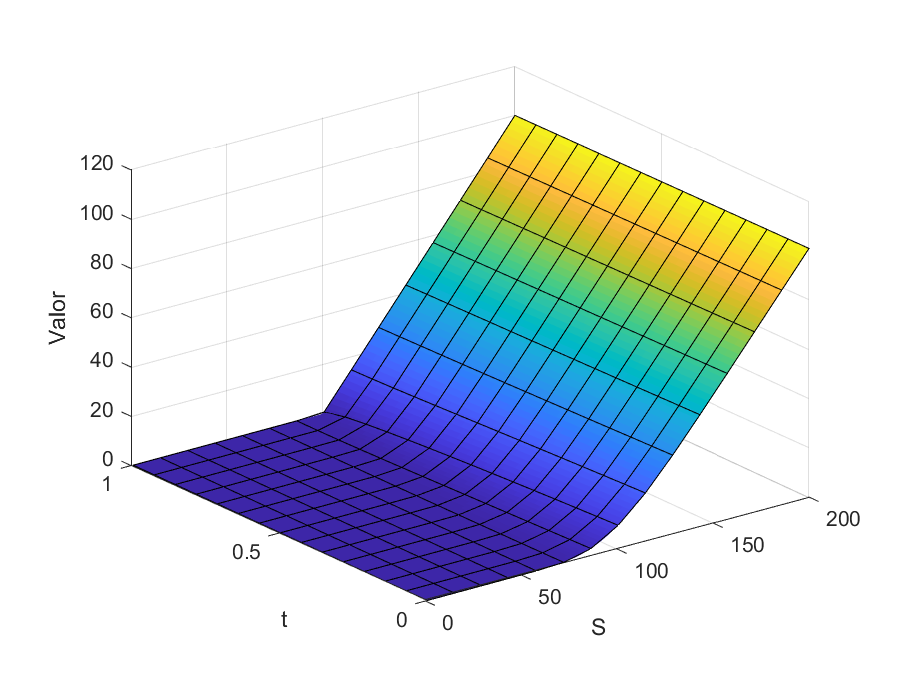
\includegraphics[width=\linewidth]{Imagenes/6_Sols/Call/Call3D.eps}
        \caption{Solución}
    \end{subfigure}
    \begin{subfigure}[b]{0.35\linewidth}
        \includegraphics[width=\linewidth]{Imagenes/6_Sols/Call/CallSFijo.eps}
        \caption{Solución con S fijo}
    \end{subfigure}
    \begin{subfigure}[b]{0.35\linewidth}
        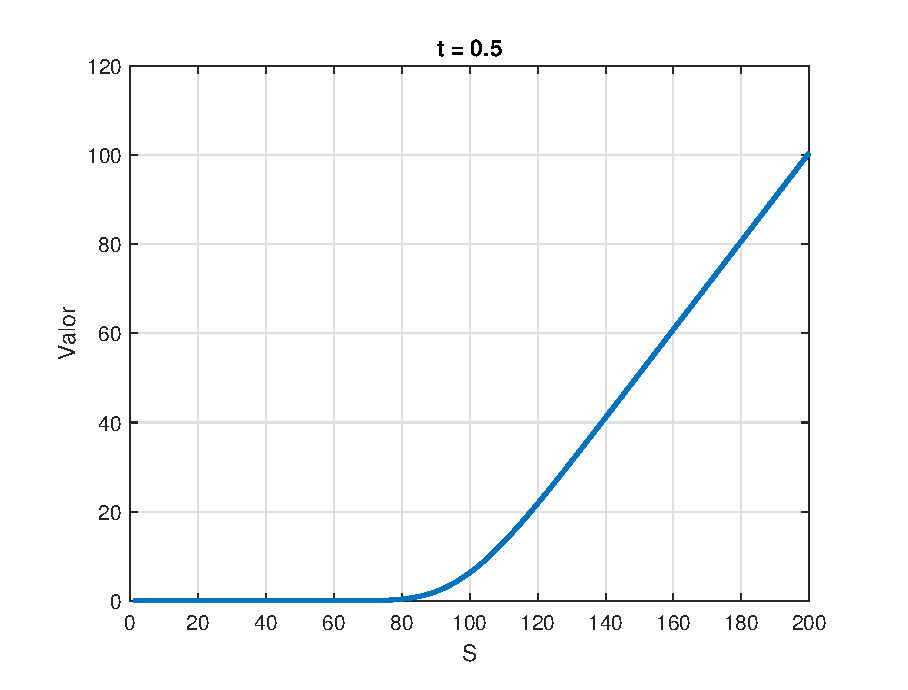
\includegraphics[width=\linewidth]{Imagenes/6_Sols/Call/CalltFIjo.eps}
        \caption{Solución con t fijo}
    \end{subfigure}
    \begin{subfigure}[b]{0.35\linewidth}
        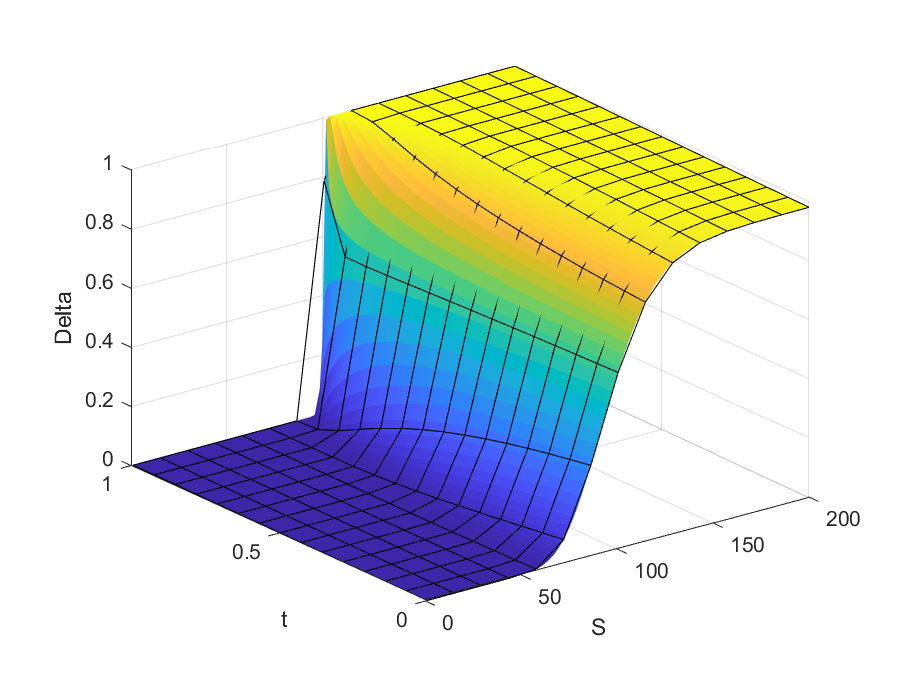
\includegraphics[width=\linewidth]{Imagenes/6_Sols/Call/Call_Delta.eps}
        \caption{Delta}
    \end{subfigure}
    \begin{subfigure}[b]{0.35\linewidth}
        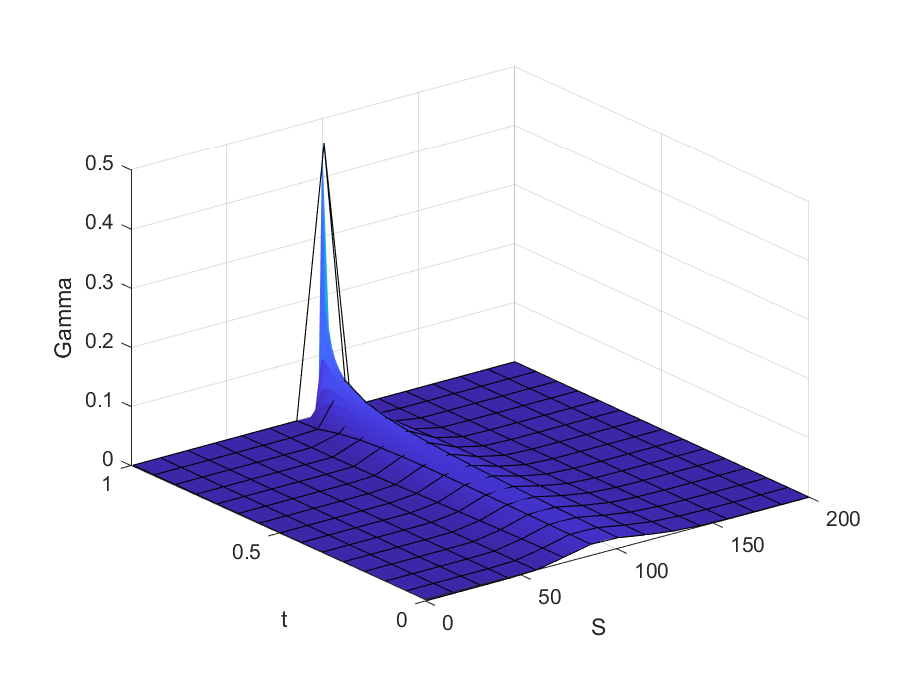
\includegraphics[width=\linewidth]{Imagenes/6_Sols/Call/Call_Gamma.eps}
        \caption{Gamma}
    \end{subfigure}
    \begin{subfigure}[b]{0.35\linewidth}
        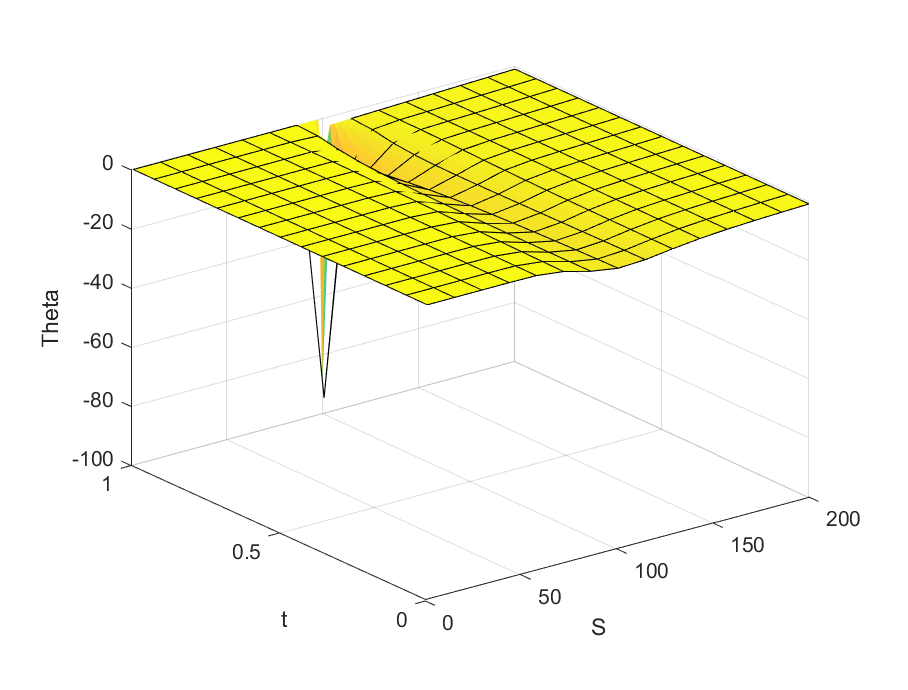
\includegraphics[width=\linewidth]{Imagenes/6_Sols/Call/Call_Theta.eps}
        \caption{Theta}
    \end{subfigure}
    \begin{subfigure}[b]{0.35\linewidth}
        \includegraphics[width=\linewidth]{Imagenes/6_Sols/Call/Call_Speed.eps}
        \caption{Speed}
    \end{subfigure}
    \begin{subfigure}[b]{0.35\linewidth}
        \includegraphics[width=\linewidth]{Imagenes/6_Sols/Call/Call_Vega.eps}
        \caption{Vega}
    \end{subfigure}
    \begin{subfigure}[b]{0.35\linewidth}
        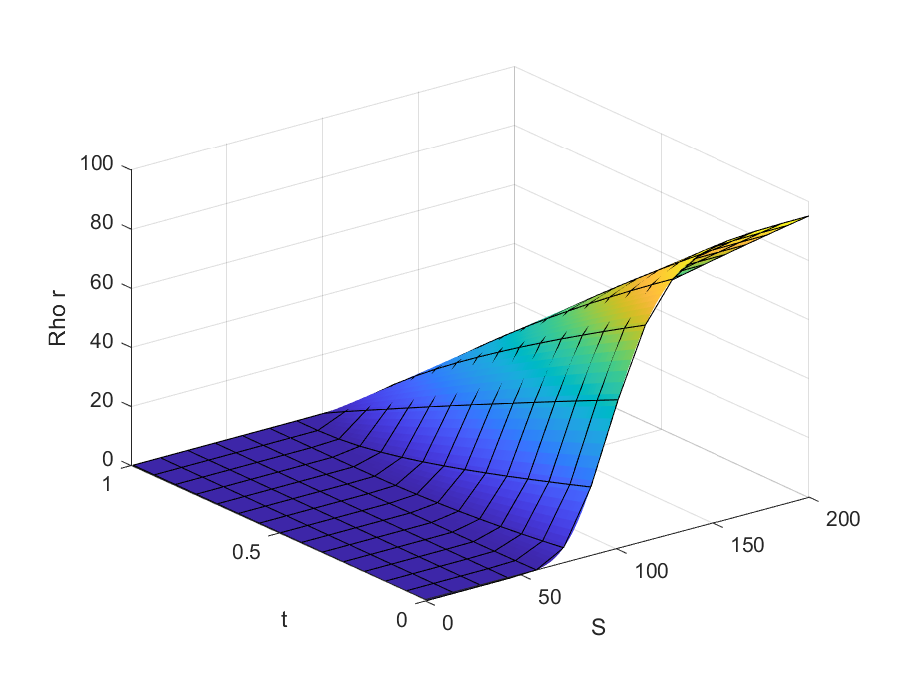
\includegraphics[width=\linewidth]{Imagenes/6_Sols/Call/Call_Rho_r.eps}
        \caption{Rho (r)}
    \end{subfigure}
    \begin{subfigure}[b]{0.35\linewidth}
        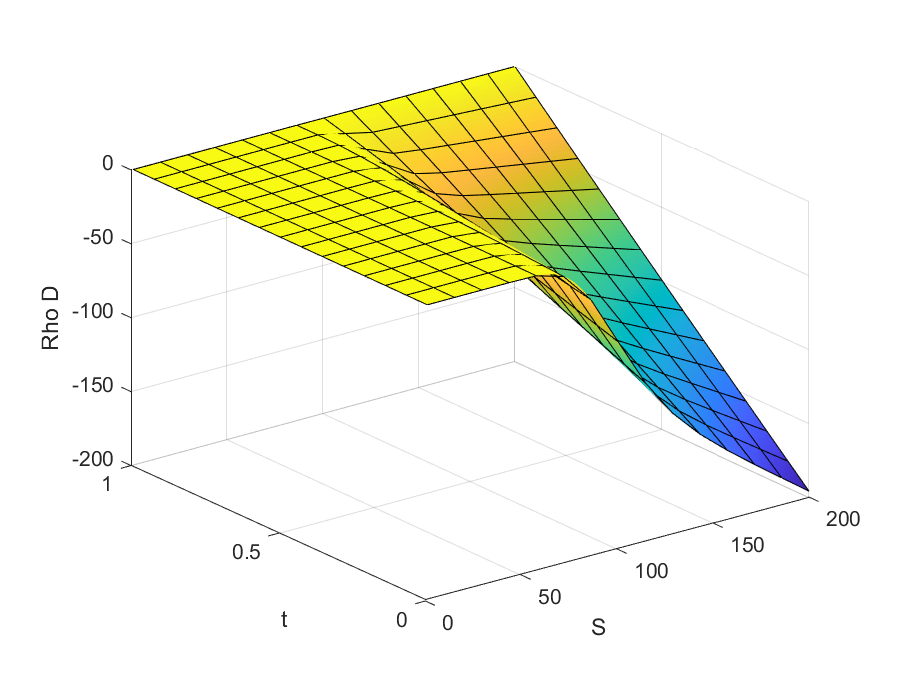
\includegraphics[width=\linewidth]{Imagenes/6_Sols/Call/Call_Rho_D.eps}
        \caption{Rho (D)}
    \end{subfigure}
\end{figure}


\subsubsection{Put option}
\begin{figure}[H]
    \centering
    \begin{subfigure}[b]{0.35\linewidth}
        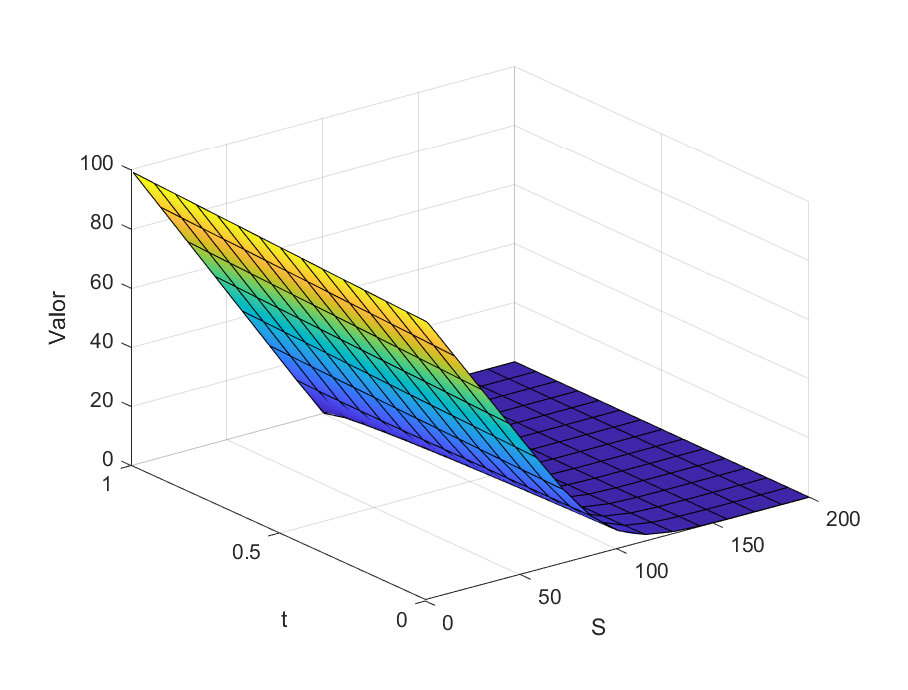
\includegraphics[width=\linewidth]{Imagenes/6_Sols/Put/Put3D.eps}
        \caption{Solución}
    \end{subfigure}
    \begin{subfigure}[b]{0.35\linewidth}
        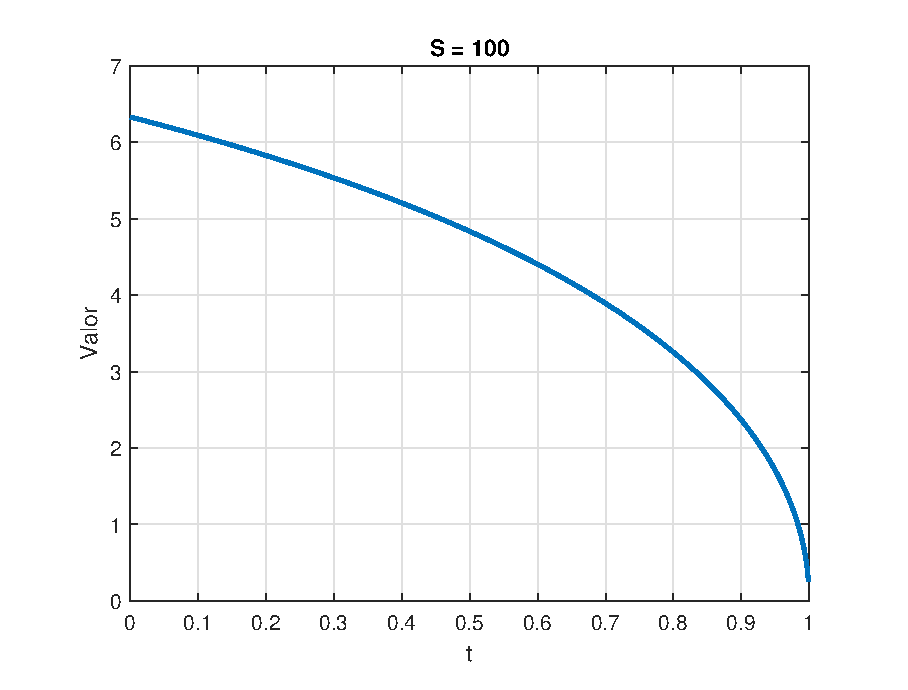
\includegraphics[width=\linewidth]{Imagenes/6_Sols/Put/PutSFijo.eps}
        \caption{Solución con S fijo}
    \end{subfigure}
    \begin{subfigure}[b]{0.35\linewidth}
        \includegraphics[width=\linewidth]{Imagenes/6_Sols/Put/PuttFIjo.eps}
        \caption{Solución con t fijo}
    \end{subfigure}
    \begin{subfigure}[b]{0.35\linewidth}
        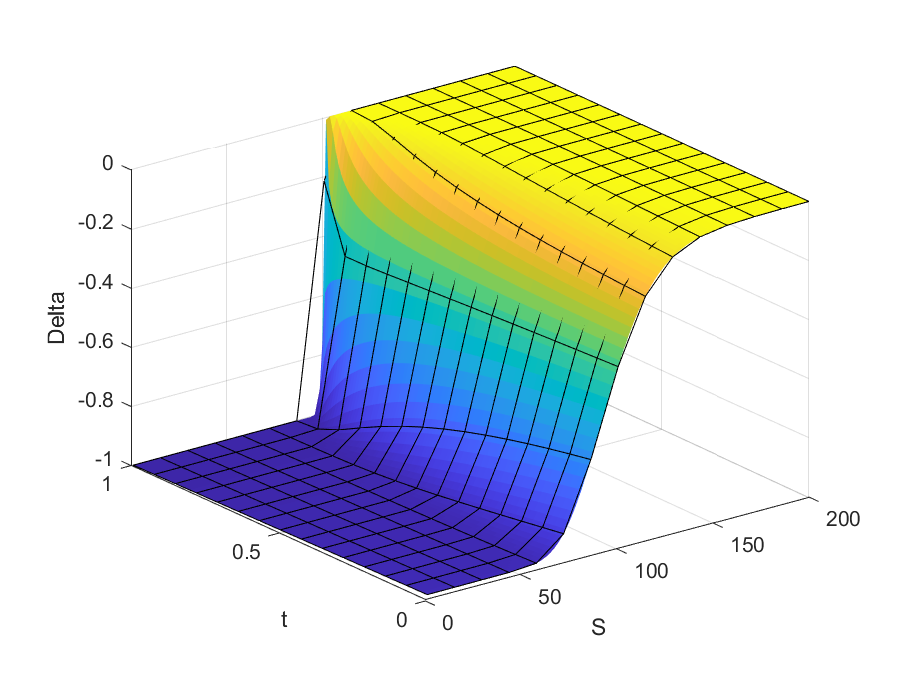
\includegraphics[width=\linewidth]{Imagenes/6_Sols/Put/Put_Delta.eps}
        \caption{Delta}
    \end{subfigure}
    \begin{subfigure}[b]{0.35\linewidth}
        \includegraphics[width=\linewidth]{Imagenes/6_Sols/Put/Put_Gamma.eps}
        \caption{Gamma}
    \end{subfigure}
    \begin{subfigure}[b]{0.35\linewidth}
        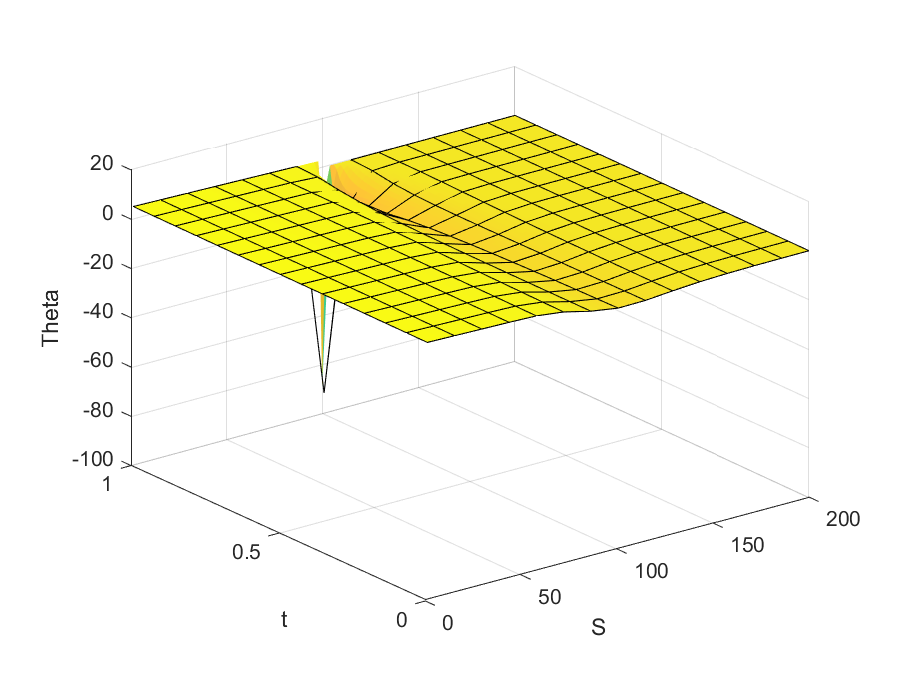
\includegraphics[width=\linewidth]{Imagenes/6_Sols/Put/Put_Theta.eps}
        \caption{Theta}
    \end{subfigure}
    \begin{subfigure}[b]{0.35\linewidth}
        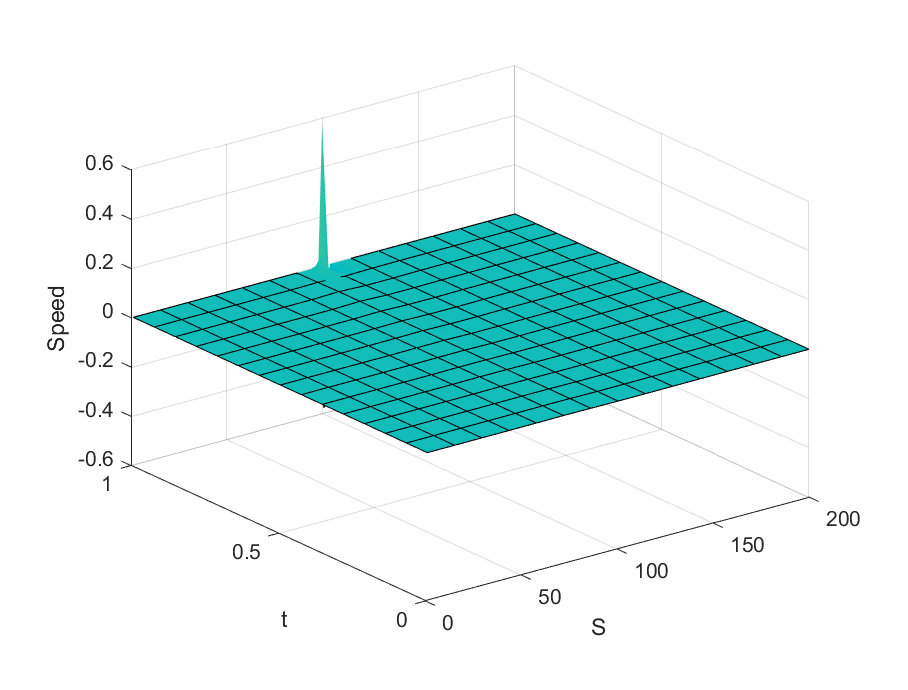
\includegraphics[width=\linewidth]{Imagenes/6_Sols/Put/Put_Speed.eps}
        \caption{Speed}
    \end{subfigure}
    \begin{subfigure}[b]{0.35\linewidth}
        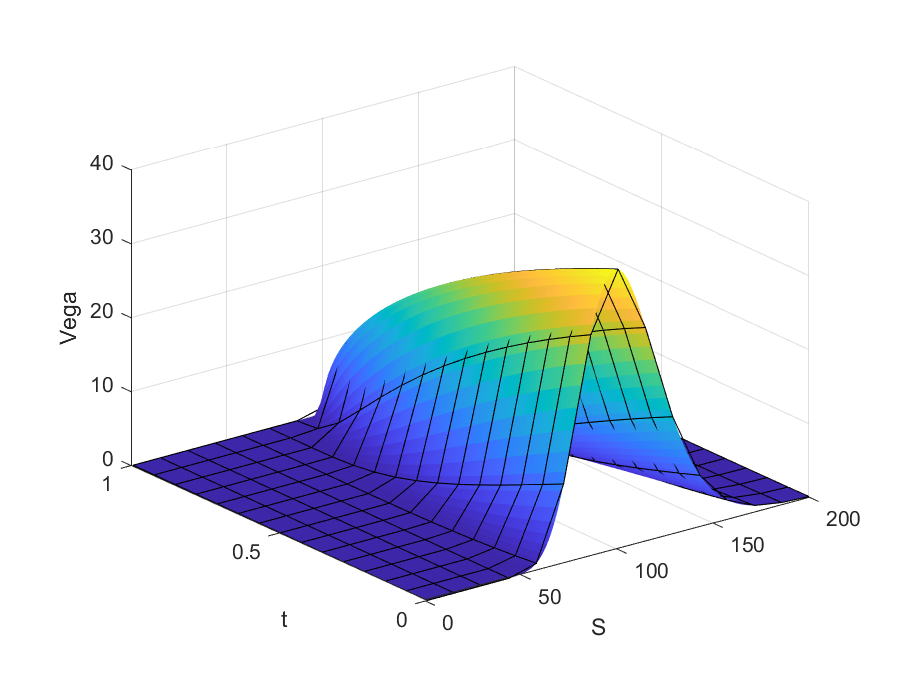
\includegraphics[width=\linewidth]{Imagenes/6_Sols/Put/Put_Vega.eps}
        \caption{Vega}
    \end{subfigure}
    \begin{subfigure}[b]{0.35\linewidth}
        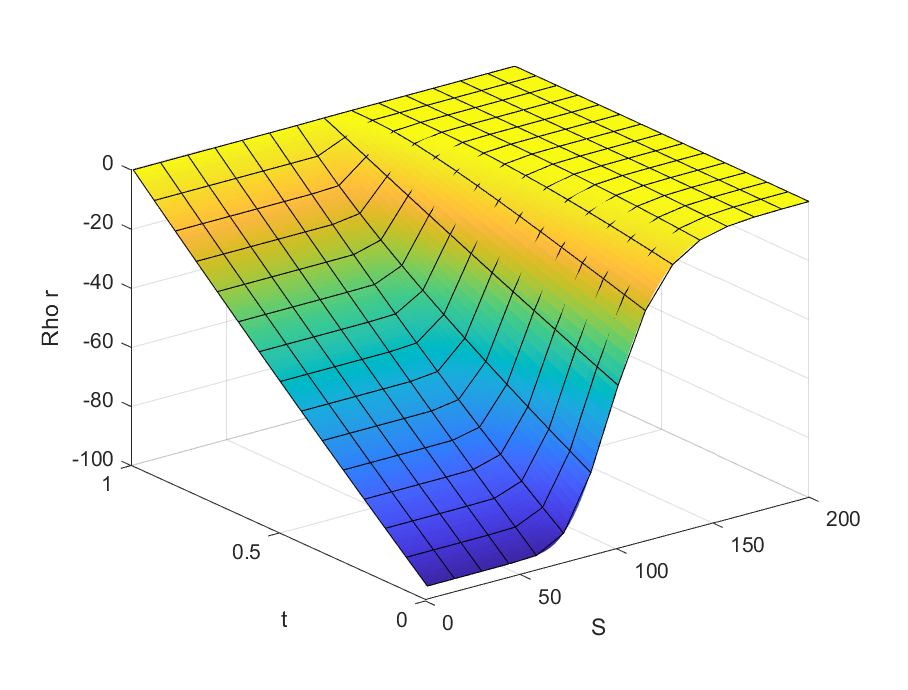
\includegraphics[width=\linewidth]{Imagenes/6_Sols/Put/Put_Rho_r.eps}
        \caption{Rho (r)}
    \end{subfigure}
    \begin{subfigure}[b]{0.35\linewidth}
        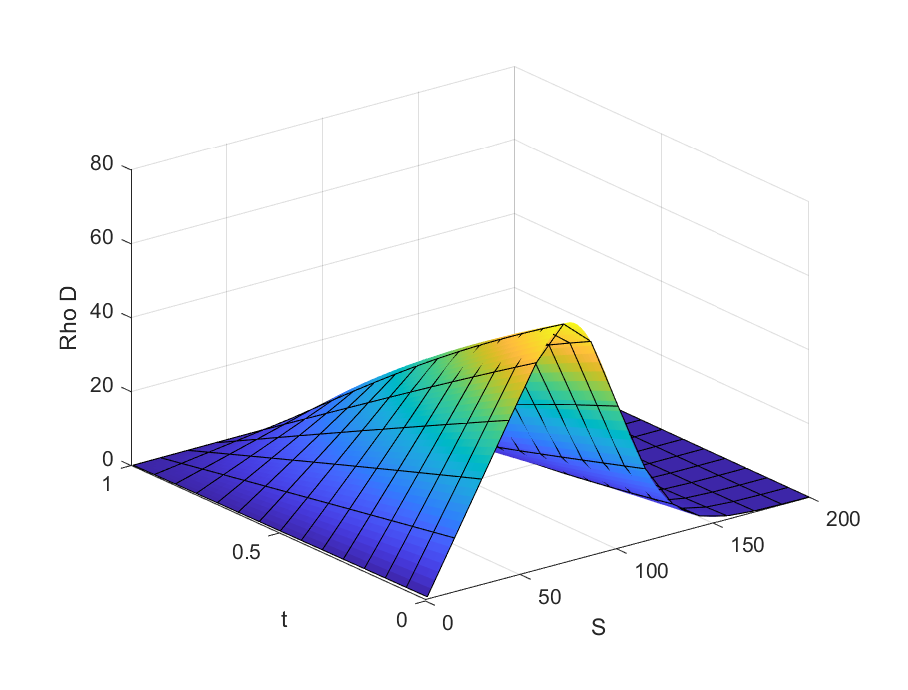
\includegraphics[width=\linewidth]{Imagenes/6_Sols/Put/Put_Rho_D.eps}
        \caption{Rho (D)}
    \end{subfigure}
\end{figure}



\subsubsection{Binary Call option}
\begin{figure}[H]
    \centering
    \begin{subfigure}[b]{0.35\linewidth}
        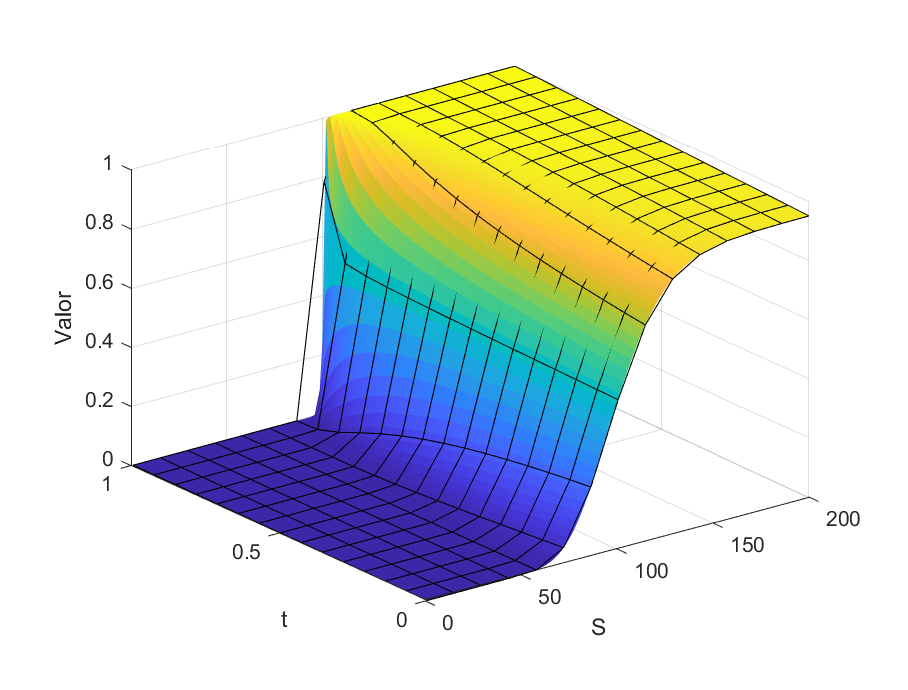
\includegraphics[width=\linewidth]{Imagenes/6_Sols/Binary_Call/BinaryCall3D.eps}
        \caption{Solución}
    \end{subfigure}
    \begin{subfigure}[b]{0.35\linewidth}
        \includegraphics[width=\linewidth]{Imagenes/6_Sols/Binary_Call/BinaryCallSFijo.eps}
        \caption{Solución con S fijo}
    \end{subfigure}
    \begin{subfigure}[b]{0.35\linewidth}
        \includegraphics[width=\linewidth]{Imagenes/6_Sols/Binary_Call/BinaryCalltFIjo.eps}
        \caption{Solución con t fijo}
    \end{subfigure}
    \begin{subfigure}[b]{0.35\linewidth}
        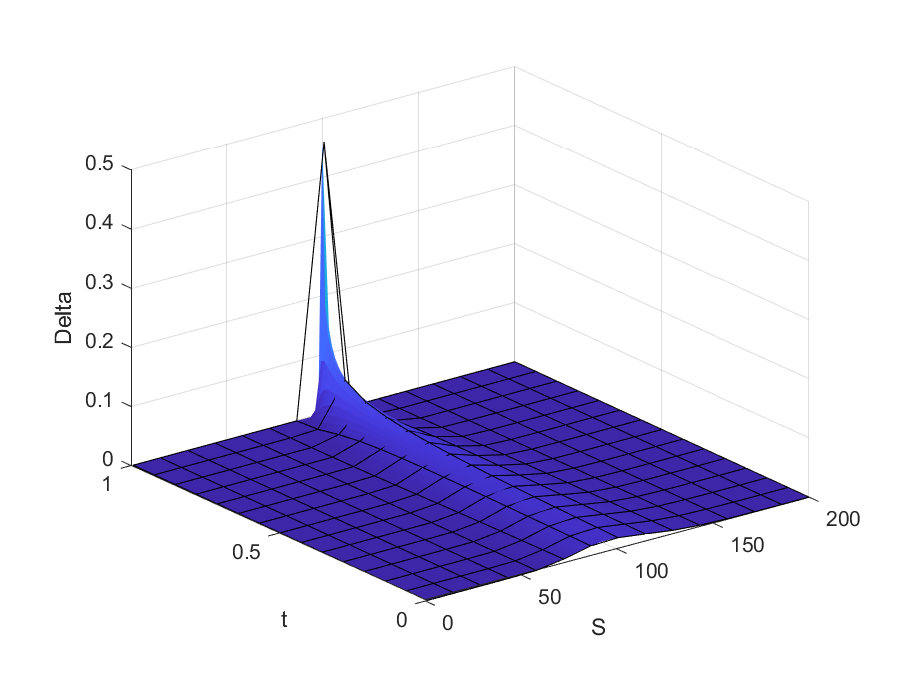
\includegraphics[width=\linewidth]{Imagenes/6_Sols/Binary_Call/Binary_Call_Delta.eps}
        \caption{Delta}
    \end{subfigure}
    \begin{subfigure}[b]{0.35\linewidth}
        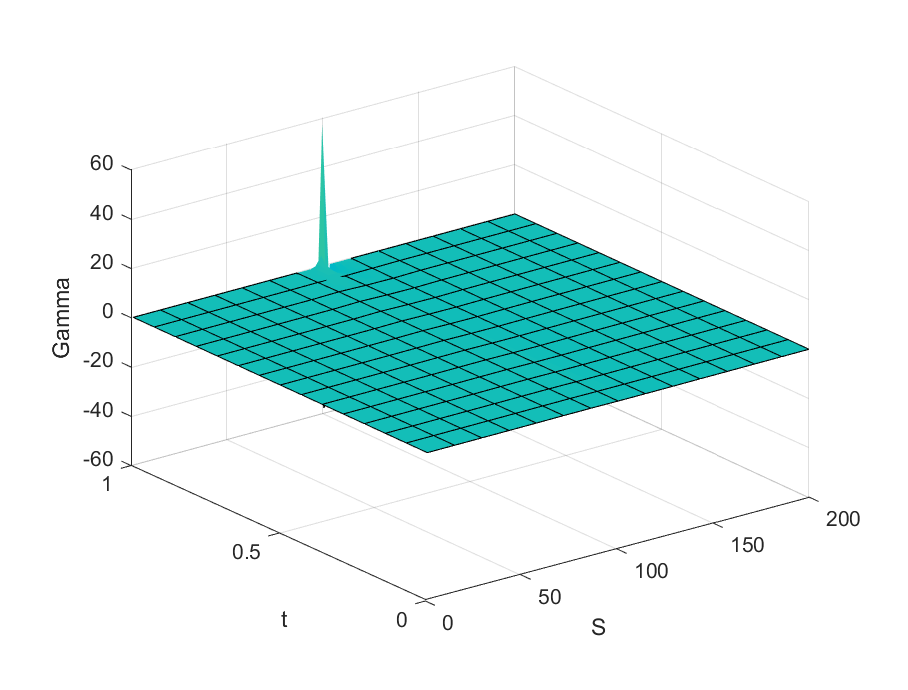
\includegraphics[width=\linewidth]{Imagenes/6_Sols/Binary_Call/Binary_Call_Gamma.eps}
        \caption{Gamma}
    \end{subfigure}
    \begin{subfigure}[b]{0.35\linewidth}
        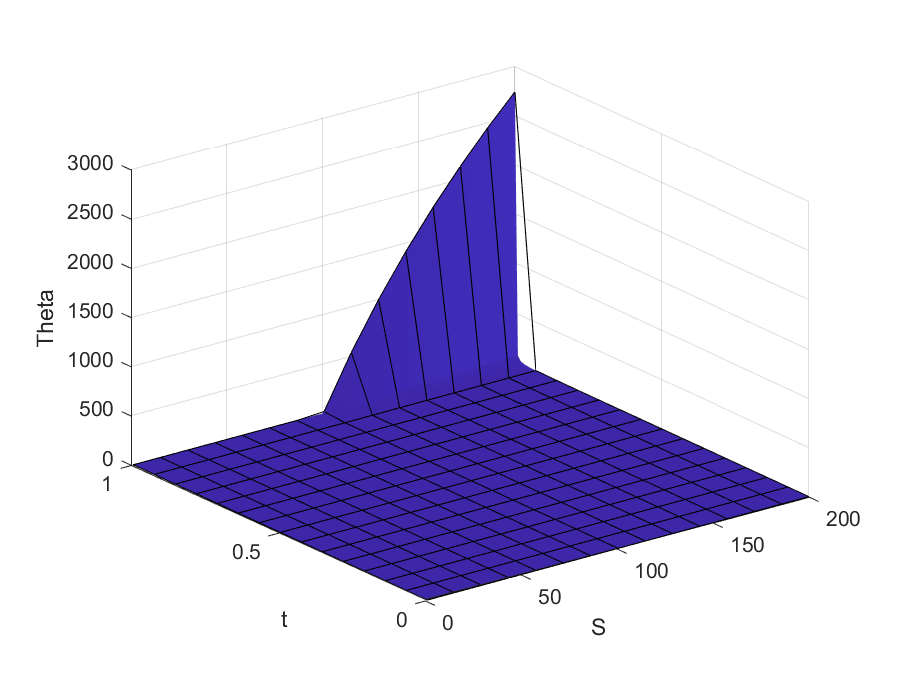
\includegraphics[width=\linewidth]{Imagenes/6_Sols/Binary_Call/Binary_Call_Theta.eps}
        \caption{Theta}
    \end{subfigure}
    \begin{subfigure}[b]{0.35\linewidth}
        \includegraphics[width=\linewidth]{Imagenes/6_Sols/Binary_Call/Binary_Call_Speed.eps}
        \caption{Speed}
    \end{subfigure}
    \begin{subfigure}[b]{0.35\linewidth}
        \includegraphics[width=\linewidth]{Imagenes/6_Sols/Binary_Call/Binary_Call_Vega.eps}
        \caption{Vega}
    \end{subfigure}
    \begin{subfigure}[b]{0.35\linewidth}
        \includegraphics[width=\linewidth]{Imagenes/6_Sols/Binary_Call/Binary_Call_Rho_r.eps}
        \caption{Rho (r)}
    \end{subfigure}
    \begin{subfigure}[b]{0.35\linewidth}
        \includegraphics[width=\linewidth]{Imagenes/6_Sols/Binary_Call/Binary_Call_Rho_D.eps}
        \caption{Rho (D)}
    \end{subfigure}
\end{figure}


\subsubsection{Binary Put option}
\begin{figure}[H]
    \centering
    \begin{subfigure}[b]{0.35\linewidth}
        \includegraphics[width=\linewidth]{Imagenes/6_Sols/Binary_Put/BinaryPut3D.eps}
        \caption{Solución}
    \end{subfigure}
    \begin{subfigure}[b]{0.35\linewidth}
        \includegraphics[width=\linewidth]{Imagenes/6_Sols/Binary_Put/BinaryPutSFijo.eps}
        \caption{Solución con S fijo}
    \end{subfigure}
    \begin{subfigure}[b]{0.35\linewidth}
        \includegraphics[width=\linewidth]{Imagenes/6_Sols/Binary_Put/BinaryPuttFIjo.eps}
        \caption{Solución con t fijo}
    \end{subfigure}
    \begin{subfigure}[b]{0.35\linewidth}
        \includegraphics[width=\linewidth]{Imagenes/6_Sols/Binary_Put/Binary_Put_Delta.eps}
        \caption{Delta}
    \end{subfigure}
    \begin{subfigure}[b]{0.35\linewidth}
        \includegraphics[width=\linewidth]{Imagenes/6_Sols/Binary_Put/Binary_Put_Gamma.eps}
        \caption{Gamma}
    \end{subfigure}
    \begin{subfigure}[b]{0.35\linewidth}
        \includegraphics[width=\linewidth]{Imagenes/6_Sols/Binary_Put/Binary_Put_Theta.eps}
        \caption{Theta}
    \end{subfigure}
    \begin{subfigure}[b]{0.35\linewidth}
        \includegraphics[width=\linewidth]{Imagenes/6_Sols/Binary_Put/Binary_Put_Speed.eps}
        \caption{Speed}
    \end{subfigure}
    \begin{subfigure}[b]{0.35\linewidth}
        \includegraphics[width=\linewidth]{Imagenes/6_Sols/Binary_Put/Binary_Put_Vega.eps}
        \caption{Vega}
    \end{subfigure}
    \begin{subfigure}[b]{0.35\linewidth}
        \includegraphics[width=\linewidth]{Imagenes/6_Sols/Binary_Put/Binary_Put_Rho_r.eps}
        \caption{Rho (r)}
    \end{subfigure}
    \begin{subfigure}[b]{0.35\linewidth}
        \includegraphics[width=\linewidth]{Imagenes/6_Sols/Binary_Put/Binary_Put_Rho_D.eps}
        \caption{Rho (D)}
    \end{subfigure}
\end{figure}
















\cleardoublepage
%\includepdf[
    pages=1-4,
    nup=1x2,
    landscape=false,
    scale=0.9,
    offset=0 0,
    frame=false
]{Imagenes/3_Aleatoriedad/6-CalculoIto2425.pdf}







\end{document}